% ============================================== %
% Author: Alessio Bandiera
%
% Thesis Title: ?
% 
% Bachelor of Science in Computer Science, Sapienza University of Rome.
%
% https://github.com/aflaag/?
%
% ============================================== %

% Document Class
\documentclass[binding=0.6cm, noexaminfo]{sapthesis}

% Packages
\usepackage{microtype}
\usepackage[english]{babel}
\usepackage[utf8]{inputenc}
\usepackage{csquotes}
\usepackage{hyperref}
\usepackage{listings}
\usepackage[dvipsnames]{xcolor}
\usepackage{xspace}
\usepackage{geometry} 
\usepackage{caption}  
\usepackage[edges]{forest}
\usepackage{subcaption}
\usepackage{float}    
\usepackage{lipsum}  
\usepackage{xargs}              
\usepackage{booktabs}
\usepackage{graphicx}
\usepackage{makecell}
\usepackage{booktabs}
\usepackage{tabularx}
\usepackage{longtable}
\usepackage{threeparttable}
\usepackage{amsthm}
\usepackage{amssymb}
\usepackage{cleveref}
\usepackage[Algoritmo]{algorithm}      
\usepackage{algpseudocode}
\usepackage[colorinlistoftodos,prependcaption,textsize=tiny]{todonotes}

\usepackage[
  backend=bibtex,
  style=numeric,
  sorting=none,
  minnames=3,
  minalphanames=3
]{biblatex}

% \nocite{*}

% Commands and Settings
\newcommandx{\unsure}[2][1=]{\todo[linecolor=red,backgroundcolor=red!25,bordercolor=red,#1]{#2}}
\newcommandx{\change}[2][1=]{\todo[linecolor=blue,backgroundcolor=blue!25,bordercolor=blue,#1]{#2}}
\newcommandx{\info}[2][1=]{\todo[linecolor=OliveGreen,backgroundcolor=OliveGreen!25,bordercolor=OliveGreen,#1]{#2}}
\newcommandx{\improvement}[2][1=]{\todo[linecolor=Plum,backgroundcolor=Plum!25,bordercolor=Plum,#1]{#2}}
\newcommandx{\thiswillnotshow}[2][1=]{\todo[disable,#1]{#2}}
\newcolumntype{L}[1]{>{\raggedright\arraybackslash}p{#1}}
\newcounter{boxlblcounter}  
\newcommand{\makeboxlabel}[1]{\fbox{#1.}\hfill}
\newenvironment{boxlabel}
  {\begin{list}
    {\arabic{boxlblcounter}}
    {\usecounter{boxlblcounter}
     \setlength{\labelwidth}{3em}
     \setlength{\labelsep}{0em}
     \setlength{\itemsep}{2pt}
     \setlength{\leftmargin}{1.5cm}
     \setlength{\rightmargin}{2cm}
     \setlength{\itemindent}{0em} 
     \let\makelabel=\makeboxlabel
    }
  }
{\end{list}}
\lstdefinestyle{myStyle}{
    belowcaptionskip=1\baselineskip,
    breaklines=true,
    numberstyle=\tiny\color{gray},
    captionpos=b,
    frame=tb,
    basicstyle=\footnotesize\ttfamily,
    keywordstyle=\bfseries\color{green!40!black},
    commentstyle=\itshape\color{blue!40!black},
    identifierstyle=\color{black},
    backgroundcolor=\color{white},
}
\lstset{style=mystyle}

\setlength{\parindent}{0pt}
\setlength{\parskip}{5pt}

% Metadata
\hypersetup{pdftitle={Thesis},pdfauthor={Alessio Bandiera}, urlcolor=black, linkcolor=black, colorlinks=true}
\title{TODO Titolo}
\author{Alessio Bandiera}
\IDnumber{1985878}
\course{Bachelor's Degree in Computer Science}
\courseorganizer{Faculty of Information Engineering, Computer Science and Statistics}
\AcademicYear{2023/2024}
\advisor{Prof. Ivano Salvo}
% \coadvisor{Prof. Massimo Lauria}
\authoremail{alessio.bandiera02@gmail.com}
\copyyear{2024}
\thesistype{Bachelor's Thesis}

% % ================== CUSTOM ENVIRONMENTS ==================
%
% \newtheorem{lemma}{Lemma}[chapter]
% \newtheorem{theorem}{Theorem}[chapter]
% \newtheorem{proposition}{Proposition}[chapter]
% \newtheorem{corollary}{Corollary}[chapter]
%
% \theoremstyle{definition}
% \newtheorem{claimlemma}{Claim}[lemma]
% \newtheorem{claimtheorem}{Claim}[theorem]
% \newtheorem{definition}{Definition}[chapter]
%
% % ================== CUSTOM MACROS ==================
%
% \renewcommand{\lnot}{\overline}
% \newcommand{\abs}[1]{\left|#1\right|}
% \newcommand{\say}[1]{\flqq\textit{#1}\frqq}
% \newcommand{\floor}[1]{\left \lfloor #1 \right \rfloor}
% \newcommand{\ceil}[1]{\left \lceil #1 \right \rceil}
% \newcommand{\abk}[1]{\left\langle#1\right\rangle}
%
% \newcommand{\TFNP}{\textsf{TFNP}\xspace}
% \newcommand{\TFNPdt}{\mathsf{TFNP}^{dt}\xspace}
%
% \newcommand{\N}{\mathbb{N}}
% \renewcommand{\P}{\mathbb{P}}
% \newcommand{\Z}{\mathbb{Z}}
% \newcommand{\F}{\mathbb{F}}
%
% \newcommand{\Res}{\mathsf{Res}}
% \newcommand{\ResP}{\mathsf{Res(\oplus)}}
% \newcommand{\NS}{\mathsf{NS}}
% \newcommand{\FNS}{\F_2\text{-}\mathsf{NS}}
% \newcommand{\enc}{\mathrm{enc}}

% ================== DOCUMENT ==================

\addbibresource{./references.bib}

\begin{document}

\lstset{language=Python}

\frontmatter

\maketitle

% ================== DEDICATION ==================
\dedication{
    TODO.
}
% ================== ABSTRACT ==================

% \begin{abstract}
    This work will discuss \textbf{computational approaches} developed to refine and improve \textit{current cancer treatments}.

    \textbf{Cancer} is one of the \textit{leading causes of death} globally, responsible for millions of deaths each year. It is a complex \textit{group of diseases} characterized by the \textit{uncontrolled growth and spread of abnormal cells} in the body, driven by a multitude of \textbf{genetic mutations}. These cells can invade surrounding tissues and, if left untreated, may spread to other parts of the body. Therefore, it is essential to search for an \textit{effective treatment}, which not only alleviates symptoms and improves the quality of life, but also addresses the underlying mechanisms of cancer.

    Over the years, \textit{various strategies} have been developed and implemented to treat cancer as effectively as possible. However, most currently employed cancer treatments have significant \textbf{side effects}, which can severely affect patients' quality of life. As a result, there is a pressing need for therapies that are not only effective in \textit{targeting cancer cells}, but also \textit{minimize harm to healthy tissues}, thereby improving the patient's overall experience during treatment.

    This work will focus specifically on one type of treatment: \textbf{targeted therapies}, which have shown significant results in recent years, both in terms of \textit{reducing side effects} and \textit{improving treatment efficacy}. Targeted therapies, as the name suggests, are designed to focus on specific molecules or pathways involved in cancer growth and progression. By precisely \textbf{targeting} these elements, targeted therapies aim to disrupt the cancer's ability to proliferate, while \textit{minimizing damage} to healthy cells, resulting in improved treatment outcomes and fewer side effects.

    However, \textbf{identifying effective targets} is not straightforward, as it depends on a variety of factors. In fact, throughout the years, numerous studies have attempted to differentiate between the \textit{vast number of mutations} that occur in cancer, aiming to identify \textit{the most relevant} ones for tumor treatment.

    Fortunately, certain \textbf{phenomena in genomic data} have been identified that could potentially be leveraged to simplify the search in this field. This work will explore the \textbf{computational approaches} adopted in recent years, the challenges this search presents, and the \textit{genomic characteristics} that newly developed algorithms leverage to \textbf{classify mutations efficiently}.

    The first chapter of this work will provide an \textbf{overview of cancer}, exploring its causes, current treatment options, and a more detailed examination of \textit{targeted therapies}. The second chapter will highlight the challenges associated with \textbf{differentiating} among the vast number of mutations involved in cancer and will \textit{introduce the studies} that will be analyzed throughout this work, focusing specifically on how they \textbf{mathematically formulated} biological phenomena observed \textit{statistically} in genomic data. The third chapter will delve deeper into the \textbf{algorithms} employed by the discussed studies, and explain how they employed their own \textit{metrics}. Finally, the last chapter will address \textbf{additional considerations} regarding the studies presented.
\end{abstract}

\let\cleardoublepage\clearpage


\cleardoublepage

\tableofcontents
\let\cleardoublepage\clearpage

\hypersetup{colorlinks=true, linkcolor=blue, citecolor=red}


\mainmatter

% ================== CHAPTERS ==================
\chapter{Introduction} \label{chap:introduction}

placeholder. \todo{abstract di tutta la tesi}

\section{Cancer}

\subsection{Overview} \todo{ho l'impressione che qui manca qualcosa, poco, ma qualcosa}

Cancer is a group of diseases characterized by uncontrolled cell proliferation, which allows cells to infiltrate into organs and tissues, thereby altering their functions and structure. There are more than 100 types of cancer, which can be grouped into broader categories such as \href{https://en.wikipedia.org/wiki/Carcinoma}{carcinomas}, \href{https://en.wikipedia.org/wiki/Sarcoma}{sarcomas}, \href{https://en.wikipedia.org/wiki/Leukemia}{leukemias} and others \cite{cancer1}.

Estimates predicted more than 2 million new cases of cancer of any site in the United States in 2024, with over 600,000 deaths \cite{cancer4}. According to SEER \cite{seer} 22, cancer is most frequently diagnosed among individuals aged 65-74, who also represent the age group with the highest cancer-related mortality, accounting for approximately 30\% of cases in both diagnoses and deaths \cite{cancer5}.

Cancer is often preceded by a range of symptoms, some of which may be subtle or easily overlooked. Possible signs and symptoms include persistent coughing, changes in bowel habits, unexplained bleeding, lumps, unexplained weight loss, persistent pain, yellowing or itchy skin, and feeling tired or unwell without a clear reason \cite{cancer3}.

The exponential growth of cancer is driven by mutations in cellular DNA, which encodes the instructions for cell development and multiplication, therefore errors in these instructions can lead to cancerous transformation. These genetic mutations can arise from several factors, including random chance or exposure to carcinogens \cite{cancer2}. These and other causes will be discussed in the following sections.

\subsection{Causes}

The development of cancer is a complex, \textit{multistep process} influenced by various factors, making it too simplistic to attribute cancer to a single cause. While genetic mutations can occur randomly through errors in DNA during cell division, or be inherited from a parent \cite{cancer2}, many agents --- such as radiation, chemicals, and viruses --- have been found to induce cancer.

Radiation and many chemical carcinogens work by damaging DNA and \textit{causing mutations}. These are known as \textbf{initiating agents} because they trigger genetic changes that lead to cancer. For example, solar ultraviolet radiation, chemicals in tobacco smoke, and \href{https://en.wikipedia.org/wiki/Aflatoxin}{\textit{aflatoxin}} are well-documented carcinogens. Tobacco smoke, in particular, is a major cause of lung cancer and is also linked to cancers of the oral cavity, throat, larynx, esophagus, and other areas. It is estimated that smoking contributes to a significant portion of all cancer deaths.

In contrast, some carcinogens --- known as \textbf{tumor promoters} --- facilitate cancer development by \textit{stimulating cell proliferation} rather than by inducing mutations. Tumor formation in animal models typically require both an initiating agent and a promoter to facilitate the growth of mutated cells. For instance, hormones (especially estrogens) play a role as tumor promoters in certain cancers.

Additionally, some viruses are known to cause cancer in both animals and humans, such as those linked to liver cancer and cervical carcinoma. These viral-induced cancers highlight the broader impact of carcinogens and underscore their role in both viral and non-viral cancer development \cite{nih_cancer_dev}.

In summary, the various ways in which different factors contribute to cancer emphasize the complexity of the disease and underscore the importance of developing effective treatment approaches, which will be explored in later sections.

\subsection{Mutations in cancer development}

The fundamental feature of cancer development is \textbf{tumor clonality}, meaning tumors often develop from single cells that start to proliferate abnormally. However, the clonal origin of tumors does not mean that the initial progenitor cell had all the features of a cancer cell from the start. Instead, cancer evolves through a multistep process in which cells \textit{gradually acquire malignant characteristics} through a series of \textbf{alterations}. This multistep nature is indicated by the fact that most cancers develop later in life. For example, the incidence of colon cancer increases markedly with age, showing a dramatic rise as individuals grow older. This steep age-related increase suggests that cancer typically results from \textbf{multiple abnormalities} accumulated over many years.

At the cellular level, cancer development is viewed as a process of mutation and selection for cells with progressively greater abilities to proliferate, survive, invade, and metastasize. The first stage, known as \textbf{tumor initiation}, involves a genetic alteration that triggers abnormal growth in a single cell, leading to the expansion of a population of clonally derived tumor cells. \textbf{Tumor progression}, continues as \textit{additional mutations} arise within this cell population, with some mutations providing a selective advantage. As a result, cells bearing these advantageous mutations become \textit{dominant} within the tumor, a process known as \textbf{clonal selection}. This selection continues throughout the tumor's evolution, causing it to grow more rapidly and become increasingly malignant \cite{nih_cancer_dev}.

Undoubtedly, mutations are fundamental to the development of cancer and to its progression. Therefore, to effectively combat this disease, it is essential to gain a comprehensive understanding of how these genetic alterations occur and contribute to tumor development.

\section{Targeted therapy}

\subsection{Current cancer treatment}

Research aimed at finding cancer treatment is continuously evolving due to the disease's lethality and complexity. Currently, the primary techniques used to remove, control, manage, and delay the effects of cancer include \cite{cancer_treat}:

\begin{itemize}
    \item \textit{surgery}, which involves the removal of the cancerous region and is generally reserved for solid tumors;
    \item \textit{radiotherapy}, which uses x-rays to destroy tumor cells, aiming to target the cancerous region as precisely as possible to preserve healthy tissue; however, radiotherapy can increase the risk of developing secondary tumors, such as leukemia or sarcomas, and may lead to delayed effects like dementia, amnesia, or progressive cognitive difficulties;
    \item \textit{chemotherapy}, which employs \textit{cytotoxic} drugs to block cellular division in both cancerous and healthy cells, but they can also induce side effects in rapidly renewing tissues;
    \item \textit{hormone therapy}, which alters the balance of specific hormones, potentially leading to side effects such as joint pain or osteoporosis.
\end{itemize}

Recent advancements in traditional cancer treatments like chemotherapy, radiotherapy, and surgery have contributed to a decline in cancer mortality rates over the years. However, these methods still face significant limitations, often resulting in tumor recurrence and mortality, due to their various side effects. This has prompted a shift toward \textbf{mutation-targeted therapies}, as a result of their potential to precisely target cancer cells and minimize damage to healthy cells and tissue \cite{target_therapy1, jci}.

\subsection{Overview and origin}

\textbf{Targeted therapy} is a form of cancer treatment that targets proteins responsible for the growth, division, and spread of cancer cells, and it forms the basis of \href{https://en.wikipedia.org/wiki/Personalized_medicine}{precision medicine}. The targets include growth factor receptors, signaling molecules, cell-cycle proteins, and other molecules crucial for normal tissue development and homeostasis, which often become overexpressed or altered in cancer cells, leading to their aberrant function \cite{se_tt}.

Unlike standard chemotherapy, which indiscriminately destroys both rapidly dividing cancerous and normal cells, targeted therapies specifically attack abnormal proteins produced by mutated genes. Because normal cells lack these tumor-specific mutations, targeted therapies often show a higher degree of selectivity, causing fewer off-target effects and achieving more rapid and substantial tumor reduction \cite{jci}.

The concept of targeted therapy originates from the german Nobel Prize Paul Ehrlich's idea of a \curlyquotes{\textit{magic bullet}} \cite{ehrlich}, when he envisioned a chemical capable of specifically targeting microorganisms. Over a century later, advances in molecular biology enhanced our understanding of the mechanisms behind cancer initiation, promotion, and progression. This progress led to the development of treatments that can interfere with specific molecular targets, typically proteins, linked to tumor growth and progression \cite{se_tt}.

\subsection{Therapy types}

Most types of targeted therapy consist of \textbf{small-molecule drugs}, which are used for targets located inside cells because their small size allows them to enter cells easily, and \textbf{monoclonal antibodies}, which are laboratory-produced proteins engineered to bind to specific targets on cancer cells. Some monoclonal antibodies help the immune system identify and destroy cancer cells by marking them, while others directly inhibit the growth of cancer cells or induce their self-destruction, and still others deliver toxins directly to cancer cells \cite{target_therapy1}.

Most targeted therapies treat cancer by interfering with specific proteins that promote tumor growth and spread. This approach differs from chemotherapy, which often kills all rapidly dividing cells. The following are the different approaches that targeted therapy employs \cite{target_therapy1}.

\begin{itemize}
    \item \textit{Immunotherapy}. Cancer cells can often evade detection by the immune system. Certain targeted therapies mark cancer cells, making them easier for the immune system to identify and destroy, while others enhance the immune system's ability to fight cancer more effectively.
    \item \textit{Signal interruption}. Targeted therapies can interrupt signals that cause cancer cells to grow and divide uncontrollably. Cells normally divide in response to specific signals binding to proteins on their surface. However, some cancer cells present changes in the proteins that tell them to divide without the signals. Targeted therapies can block these proteins, slowing the uncontrolled growth of cancer.
    \item \textit{Angiogenesis inhibition}. The process through which new blood vessels form is called \href{https://en.wikipedia.org/wiki/Angiogenesis}{angiogenesis}; beyond a certain size tumors need new blood vessels, thus the tumor sends signals to start angiogenesis. Some targeted therapies can disrupt the signals that trigger this process, preventing the formation of a blood supply, and restricting the tumor's size. 
    \item \textit{Cell-killing agents delivery}. Some monoclonal antibodies are combined with substances like toxins, chemotherapy drugs, or radiation. These antibodies bind to targets on the surface of cancer cells, delivering the cell-killing agents directly into the cells, causing them to die. Most importantly, cells without these targets remain unharmed.
    \item \textit{Apoptosis activation}. Cancer cells often evade the natural process of cell death, known as \href{https://en.wikipedia.org/wiki/Apoptosis}{apoptosis}, which initiates when cells become damaged or are no longer needed. Some targeted therapies can trigger apoptosis in cancer cells, leading to their death.
    \item \textit{Hormone therapy}. Some types of breast and prostate cancer require specific hormones to grow. Hormone therapies block the body's production of growth hormones or prevent them from acting on cells, including cancer cells.
\end{itemize}

The diverse strategies employed by targeted therapies highlight the innovative approaches being developed to treat cancer more precisely. As research advances, these methods will continue to evolve, potentially improving outcomes and reducing side effects compared to traditional treatments.

\subsection{Drawbacks and side effects}

Like all cancer treatment, targeted therapy also has limitations, and often works best when combined with other types of targeted therapies or additional cancer treatments like chemotherapy and radiation \cite{target_therapy1}.

In particular, developing drugs for certain targets can be challenging due to factors including the target's structural complexity, its function within the cell, or a combination of both. Moreover, cancer cells can develop resistance to targeted therapy, which may occur if the target itself mutates, rendering the therapy unable to interact with it effectively. Alternatively, resistance can arise if cancer cells adapt and find new growth mechanisms that do not rely on the target \cite{target_therapy1}.

% \todo{ho un paper con il quale è possibile espandere questa sezione ma ho tolto la sezione che avevo scritto perché non credo sia necessario (almeno per il momento) scendere così tanto nel dettaglio di questa parte}

% The following are several ways in which cancer cells can develop resistance to targeted therapy \cite{target_therapy2}.
%
% \paragraph{Direct target reactivation}
%
% One of the first and most notable successes in targeted cancer therapy was the use of \href{https://en.wikipedia.org/wiki/Imatinib}{\textit{imatinib}}, a \textit{small-molecule drug} which inhibits ABL-kinase, employed to treat chronic myelogenous leukemianitial. Studies of patients who relapsed despite imatinib treatment revealed that BCR-ABL kinase activity often reappeared. This discovery revealed a key mechanism of resistance to targeted therapy: the direct restoration of the biological function that was previously disrupted by \textit{imatinib}.
%
% Another instance is the use of potent anti-androgens such as \textit{enzalutamide} can effectively control disease even in CRPC (\textit{Castration-Resistant prostate cancer}). Notably, a prevalent mechanism of resistance to \textit{enzalutamide} involves the removal of the drug-binding domain of the androgen receptor through \href{https://en.wikipedia.org/wiki/Alternative_splicing}{alternative splicing}. Indeed, alternate splicing has been frequently observed as a method for reactivating targets in response to targeted inhibitors.
%
% Another form of on-target resistance involves the increased expression of the targeted oncoprotein through transcriptional upregulation or genomic amplification. This has been noted in melanoma, NSCLC (\textit{Non-small Cell Lung Cancer}), and prostate cancer, and can be counteracted with stronger inhibitors and blockade of downstream signaling.
%
% These examples show that restoring the biological function of targeted oncoproteins is a key mechanism by which cancer cells evade targeted therapies and overcome \href{https://en.wikipedia.org/wiki/Oncogene_addiction}{oncogene addiction}.
%
% \paragraph{Oncogenic pathway signals activation}
%
% \paragraph{Alternative oncogenic pathways engagement}
%
% \paragraph{Adaptive survival mechanisms}

As for side effects, in general, targeted molecular therapies have good toxicity profiles. However, side effects differ from person to person, even among those undergoing the same cancer treatment \cite{nih_se}, and some patients may be highly sensitive to these drugs and may develop specific and severe toxicities \cite{se_tt}.

The most common side effects of targeted therapy are diarrhea and liver issues, but they may also include problems with blood clotting and wound healing, high blood pressure, fatigue, mouth sores, nail changes, loss of hair color, and skin problems. In rare cases, a perforation may occur in the wall of the esophagus, stomach, small intestine, colon, rectum, or gallbladder. Medications are available to manage many of these side effects, either by preventing them or treating them once they arise. Additionally, most side effects of targeted therapy subside after the treatment is completed \cite{target_therapy1}.

In conclusion, although targeted therapy shows promise with generally manageable side effects, it has limitations such as potential drug resistance and varying individual responses. Effective management of these side effects and ongoing research are essential to improving treatment outcomes and patient care.

% \paragraph{DAEs}
%
% Targeted therapies and immunotherapies are linked to a variety of \textit{Dermatologic Adverse Events} (DAEs) due to the involvement of common signaling pathways in both malignant processes and the normal functions of the epidermis and dermis. Dermatologic toxicities can affect the skin, oral mucosa, hair, and nails.
%
% The most frequent DAE is \textit{acneiform rash}, seen in multiple of patients undergoing treatment that include epidermal growth factor receptor (EGFR) inhibitors. BRAF inhibitors are known to cause secondary skin tumors, including \textit{squamous cell carcinoma} and \textit{keratoacanthomas}, and can also alter pre-existing pigmented lesions, and induce hand-foot skin reactions. (\textit{Immune checkpoint inhibitors} (ICIs) typically lead to nonspecific \textit{maculopapular rash}, but can also cause \textit{psoriatic} lesions, \textit{lichenoid dermatitis}, \textit{xerosis}, and \textit{pruritus}.
%
% Among the oral mucosal toxicities from targeted therapies, \textit{oral mucositis} is most frequent with mammalian Target of Rapamycin (mTOR) inhibitors, followed by \textit{stomatitis} from multikinase angiogenesis and HER inhibitors, geographic tongue, and \textit{hyperpigmentation}. ICIs generally cause oral lichenoid reactions and \textit{xerostomia}.
%
% Regarding skin problems, \textit{alopecia} is a frequent side effect of both targeted and endocrine therapies. Moreover, targeted therapies can damage the nail folds, resulting in \textit{paronychia} and \textit{periungual pyogenic granuloma}. Mild \textit{onycholysis}, brittle nails, and slower nail growth may also occur \cite{skin_nails}.
%
% \paragraph{Gastrointestinal toxicity}
%
% Diarrhea serves as a dose-limiting toxicity for many small-molecule tyrosine kinase inhibitors. \href{https://en.wikipedia.org/wiki/Gefitinib}{\textit{Gefitinib}}, in particular, has been associated with significant mucosal toxicity when administered at higher doses, although the exact mechanism remains unclear. Research indicates that many patients with colorectal cancer treated with \textit{gefitinib} alongside \textit{irinotecan}, \textit{5-fluorouracil}, and \textit{leucovorin} developed a gastrointestinal syndrome characterized by abdominal pain and diarrhea, necessitating dose reductions and preventing further development of this combination \cite{se_tt}.
%
% \paragraph{Lung problems}
%
% \textit{Interstitial lung disease} (ILD) is recognized as a potential adverse effect of certain cancer chemotherapeutic agents and local radiotherapy. Recently, ILD related to \textit{gefitinib} has emerged as a significant toxicity concern. Studies reported that multiple patients with \textit{non-small cell lung cancer} (NSCLC), treated with \textit{gefitinib}, developed ILD, and the condition led to a fatal outcome in some of them. Although the exact mechanism of \textit{gefitinib}-related ILD is not fully understood, EGFR is believed to play a crucial role in maintaining and repairing epithelial tissues and regulating mucin production in the airways. \textit{Gefitinib} appears to primarily induce pulmonary side effects in patients with existing pulmonary conditions \cite{se_tt}.

\subsection{Drugs targeting mutations}

As mentioned earlier, mutations play a crucial role in the growth and development of cancer. Targeted therapy allows for precise targeting of the mutations that enable cancer to continue its progression. In particular, oncogenic gene mutations may be druggable in several ways \cite{jci}:

\begin{itemize}
    \item some oncogenic gene mutations encode proteins that are structurally or functionally different from the wild-type (WT), normal version of the protein; these differences create an opportunity for developing targeted therapies, because a drug can be designed specifically to bind to these unique features, and inhibit the protein's activity, without affecting the WT protein in healthy cells;
    \item gene mutations often result in the abnormal activation of some protein, through mechanisms like a \textit{gain-of-function mutation} or \textit{gene amplification}; although these proteins are considered druggable, the mutation does not necessarily change the protein in a way that allows for mutant-specific targeting, i.e. drugs may also target the WT version of the protein present in healthy cells, potentially leading to more side effects;
    \item some oncogenic mutations create novel molecular dependencies or vulnerabilities in cancer cells, which can be exploited by targeted therapies; these are called \textit{actionable mutations} because they provide new targets for drug development that are specific to cancer cells and do not exist in normal cells.
\end{itemize}

While truly druggable mutations in the first category are relatively rare, many overactive or amplified targets still offer effective therapeutic opportunities due to their elevated expression levels or the significant dependence of cancer cells on these specific proteins. Additionally, mutations that currently lack targeted therapy options can still function as biomarkers to guide other therapeutic decisions \cite{jci}.

Advances in targeted therapies have been significantly driven by technological progress in sequencing over the past two decades, particularly with the development of \href{https://en.wikipedia.org/wiki/Massive_parallel_sequencing}{next-generation sequencing} (NGS). The identification of both common and rare genetic mutations has launched research into targeted therapies against mutant proteins and aberrant molecular signaling pathways. Moreover, the discovery of the \href{https://en.wikipedia.org/wiki/Philadelphia_chromosome}{BCR-ABL fusion gene} and the development of the BCR-ABL inhibitor \href{https://en.wikipedia.org/wiki/Imatinib}{\textit{imatinib}} marked a breakthrough in targeted cancer therapies, leading to numerous FDA-approved drugs \cite{jci}. However, the challenge of developing targeted therapies remains difficult, particularly for mutations that affect normal and cancerous proteins alike, or those for which no targeted therapies currently exist. The complexities of druggable mutations and their effects on treatment underscore the need for ongoing research and refinement in this area. Given the importance of fully understanding the role of mutations in cancer development, in order to improve targeted therapies and cancer treatment overall, research must focus on genomic mutations and their classification. The next chapter will discuss the existence of different types of mutations and the current techniques used to classify them.

\cleardoublepage

% \chapter{Classifying mutations} \label{chap:classifying_mutations}

\textbf{Cell signaling} is the process by which cells interact with each other, themselves, or their environment. It concerns the transduction of signals, which can be chemical, or can involve various types such as pressure, temperature, or light signals \cite{cell_signaling}. \textbf{Pathways} are sequences of molecular interactions within a cell that lead to a change in the cell or the production of a specific product \cite{pathway}. These pathways have a direction in which the actions occur, with the terms \textit{upstream} and \textit{downstream} indicating the initial and final stages of these processes, respectively.

In cancer research, \textbf{signaling pathways} are of particular interest because they mediate the transduction of cell signals. Identifying and targeting the signaling pathways responsible for cancer growth could potentially halt the development of the disease. \todo{\href{https://www.ncbi.nlm.nih.gov/pmc/articles/PMC8002322/}{check this out}, also check if what i wrote is actually true, i think i read it somewhere but can't find the source right now; expand on cell signaling? expand of pathways? if yes, make subsections}

\section{Mutations}

\subsection{Passenger and driver mutations}

There are two types of mutations in cancer: \textbf{passenger mutations} and \textbf{driver mutations}. Passenger mutations do not confer direct benefits to tumor growth or development, whereas driver mutations actively contribute to cancer progression by providing an evolutionary advantage and promoting the proliferation of tumor cells. A \textbf{driver gene} is a gene that harbors at least one driver mutation, though it may also contain passenger mutations \todo{\href{https://www.aiom.it/wp-content/uploads/2019/02/20190524RM_21_Tommasi.pdf}{DO I ADD THIS AS A CITATION???}}. A driver pathway consists of at least one driver gene. Driver mutations, genes, and pathways are of significant scientific interest due to their crucial role in cancer proliferation.

Driver genes can be classified into 12 signaling pathways, which regulate cellular functions related to survival, fate, and genomic maintenance. \todo{use (and expand) this? same source as prev}

\section{Classifying mutations}

\subsection{Frequency}

To classify mutations into the two categories described, assessing their biological function is essential, though this remains a challenging task. Numerous methods exist to predict the functional impact of mutations based on \textit{a priori} knowledge. However, these approaches often fail to integrate information effectively across various mutation types and are limited by their reliance on known proteins, rendering them less effective for less-studied ones \cite{multi-dendrix}.

With the decreasing cost of DNA sequencing, it is now possible to categorize mutations by examining their frequency, as driver mutations are typically the most recurrent in patients' genomes \cite{multi-dendrix}. Indeed, key driver events, such as TP53 loss-of-function mutations, can be identified by their significantly high frequency of occurrence across a set of tumors \cite{mutex}. However, in many cases, since driver mutations are predominantly located in genes that are part of cell signaling pathways, different patients may harbor mutations in different pathway loci. Indeed, driver mutations can vary extensively between patient samples, even within the same cancer type \cite{multi-dendrix}; additionally, there is minimal overlap of mutated genes across sample pairs, even from the same patient \cite{mdpfinder}, reducing the statistical power of frequency analyses.

Moreover, multiple alternative driver alterations in different genes may lead to similar downstream effects. In such instances, the selective advantage is distributed among the alterations frequencies of these genes. In current cancer genomics studies, where the number of samples is significantly smaller than the number of genes profiled per sample, frequency-based methods lack the statistical efficacy to distinguish passenger and driver mutations \cite{mutex}. 

Therefore, studies should be conducted at the pathway level, as it is well established that different mutations can affect the same pathway across multiple samples \cite{multi-dendrix}. However, since each pathway involves multiple genes, numerous possible combinations of driver mutations could impact a crucial cancer pathway, making it computationally unfeasible to test every possible gene permutation \cite{dendrix} --- estimates suggest that the human genome contains more than 50,000 genes \cite{n-genes}. Hence, it is necessary to identify a property to leverage to conduct the research efficiently.

\subsection{Mutual exclusivity and coverage}

Most techniques developed in recent years for recognizing driver mutations leverage a statistical property observed in cancer patient data: each patient typically has a relatively small number of mutations that affect multiple pathways, thus each pathway will contain \textit{1 driver mutation on average} per sample. This concept of mutual exclusivity among driver mutations within the same pathway, as statistically observed in patient samples, is then axiomatized and employed by research algorithms designed to identify driver mutations \cite{multi-dendrix}. Additionally, mutual exclusivity \textit{does not affect different pathways}; it is a phenomenon that occurs exclusively within a single pathway. While the precise explanation for this occurrence is not yet fully understood, several hypotheses appear promising \cite{survey, mutual_exclusivity_expls, dendrix}:

\begin{itemize}
    \item one hypothesis is that mutually exclusive genes are functionally connected within a common pathway, acting on the same downstream effectors and creating functional redundancy; consequently, they would share the same selective advantage, meaning that the alteration of one mutually exclusive gene would be sufficient to disrupt their shared pathway, thereby removing the selective pressure to alter the others; this explanation, however, does not fully account for the phenomenon because the co-alteration of mutually exclusive genes should not result in negative effects on the cell.
    \item an alternative explanation is that the co-occurrence of mutually exclusive alterations is detrimental to cancer survival, leading to the elimination of cells that harbor such co-occurrences; moreover, some pairs of mutually exclusive genes could be \textit{synthetic lethal}, meaning that while the alteration of one gene may be compatible with cell survival, the simultaneous aberration of both genes would be lethal to the cell \todo{add example from survey paper?; also, use \href{https://www.nature.com/articles/s41467-020-20820-x}{example}? (mail "Risposte (parziali) alle questioni, ERG e SPOP")}.
\end{itemize}

In addition, another key property of driver pathways is \textbf{coverage}, i.e. driver genes constituting a driver pathway are frequently mutated across many samples. \todo{ho parlato tanto della mutua esclusività e poco della coverage, sembra sbilanciato ma non so veramente cosa aggiungere perché non c'è altro da dire}

Thus, \textit{a driver pathway consists of genes that are mutated in numerous patients, with mutations being approximately mutually exclusive}. It is also observed that pathways exhibiting these characteristics are generally shorter and comprised of fewer genes on average \cite{multi-dendrix}.

\section{Mutual exclusivity formalization}

\subsection{Hard and soft mutual exclusivity}

In the statistical literature, two types of mutual exclusivity are defined: \textbf{hard} and \textbf{soft}. Hard mutual exclusivity describes events that are presumed to be strictly mutually exclusive, with the null hypothesis being that any observed overlap is due to random errors. However, in this context, it is not feasible to test for hard mutual exclusivity, as this is a property observed statistically from patient data. Therefore, it is necessary to relax the constraint to soft mutual exclusivity, where two otherwise independent events overlap less than expected by chance due to some statistical interaction \cite{mutex}.

\subsection{Mutual exclusivity of a group}

Searching for the most mutually exclusive gene group is equivalent to identifying a single driver pathway, for the aforementioned reasons. For a pair of genes, soft mutual exclusivity can be assessed using the \href{https://en.wikipedia.org/wiki/Fisher\%27s_exact_test}{Fisher's exact test}. However, there is no agreed-upon method for analytically testing mutual exclusivity among more than two genes. One approach could involve checking whether each pair of genes within the group exhibits mutual exclusivity; this method, however, may be overly strict, as a gene set can exhibit a strong mutual exclusivity pattern as a whole even if no individual pairs show any \cite{mutex}.

\subsection{Dendrix}

The authors of a very well-known paper, which developed two algorithms called \curlyquotes{Dendrix} \cite{dendrix}, gave the following mathematical formalization to the properties of mutual exclusivity and coverage for a set of genes.

\begin{definition}[Mutation matrix] \label{mut_matrix_def}
    A \curlyquotes{mutation matrix} is a matrix with $m$ rows and $n$ columns, where each row represents a patient and each column represents a gene, and the entry $a_{i, j}$ is equal to 1 if and only if gene $j$ is mutated in patient $i$.
\end{definition}

\begin{example} \label{mutation_matrix}
    An example of a mutation matrix is the following:

    \begin{table}[H]
        \centering
        \begin{tabular}{c|ccc}
                  & $g_1$ & $g_2$ & $g_3$ \\
            \hline
            $p_1$ & 0 & 1 & 0 \\
            \hline
            $p_2$ & 1 & 1 & 0 \\
            \hline
            $p_3$ & 0 & 0 & 1 \\
        \end{tabular}
        \caption{A mutation matrix.}
    \end{table}
\end{example}

\begin{definition}[Coverage of a gene]
    Given a gene $g$, the \textbf{coverage of $g$} $$\Gamma(g) := \{i \mid a_{i, g} = 1\}$$ denotes the set of patients which have $g$ mutated.
\end{definition}

Under the previous definitions of mutual exclusivity, $M$ is \textbf{mutually exclusive} if no patient has more than one mutated gene, formally $$\forall g, g' \in M \quad \Gamma(g) \cap \Gamma(g') = \varnothing$$

\begin{definition}[Coverage of a set]
    Given a set of $M$ genes, the \textbf{coverage of $M$} $$\Gamma(M) := \bigcup_{g \in M}{\Gamma(g)}$$

denotes the set of patients in which at least one of the genes in $M$ is mutated.
\end{definition}

Any gene set can be thought of as a $m \times k$ submatrix of a mutation matrix $A$, up to rearranging $A$'s columns --- their order does not matter since they represent genes. Accordingly, such a submatrix is said to be \textbf{mutually exclusive} if each row contains at most one 1.

Furhermore, given a gene set $M$, the following properties are formalized:

\begin{enumerate}[label=\roman*), font=\itshape]
    \item \textit{coverage}: most patients have at least one mutation in $M$;
    \item \textit{approximate exclusivity}: most patients have exactly one mutation in $M$.
\end{enumerate}

To evaluate these two attributes, a measure that quantifies the trade-off between coverage and mutual exclusivity is introduced.

\begin{definition}[Coverage overlap] \label{cov_over}
    Given a set $M$ of genes, the \textbf{coverage overlap} is defined as follows: $$\omega(M) := \sum_{g \in M}{\abs{\Gamma(g)}} - \abs{\Gamma(M)}$$
\end{definition}

Note that the sum in \cref{cov_over} is the number of 1s in $M$'s corresponding submatrix.

\begin{example}[Coverage overlap]
    Considering the mutation matrix in \cref{mutation_matrix}, if $M=\{g_1, g_2\}$ then $$\omega(M)=\abs{\Gamma(g_1)} + \abs{\Gamma(g_2)} - \abs{\Gamma(\{g_1, g_2\})} = \abs{\{p_2\}} + \abs{\{p_1, p_2\}} - \abs{\{p_1, p_2\}} = 1 + 2 - 2 = 1$$
\end{example}

Indeed, $\omega(M)$ is the \textit{number of patients that are counted more than once in the sum}, and $\omega(M) = 0$ only if the sum equals the coverage of $M$, which means that no patient has more than one mutated gene of $M$.

\begin{definition}[Mutually exclusive set]
    A gene set $M$ is considered to be \textbf{mutually exclusive} if $\omega(M) \ge 0$ \todo{come fa ad essere negativo?}.
\end{definition}

\begin{definition}[Weight of gene set] \label{weight}
    Given a set of genes $M$, to take into account both coverage and coverage overlap, the following measure is introduced: $$W(M): = \abs{\Gamma(M)} - \omega(M) = 2 \abs{\Gamma(M)} - \sum_{g \in M} {\abs{\Gamma(g)}}$$
\end{definition}

Note that $W(M) = \Gamma(M)$ when $M$ is mutually exclusive. In order to find an optimal gene set, the following problem has to be solved:

\begin{displayquote}\label{mwsp}
    \textbf{Maximum Weight Submatrix Problem}: Given an $m \times n$ mutation matrix $A$, and an integer $k > 0$, find a $m \times k$ submatrix of $A$ that maximizes $W(M)$.
\end{displayquote}

Finding the solution to this problem is computationally difficult even for small values of $k$ (e.g. there are $\approx 10^{23}$ subsets of size $k = 6$ of 20,000 genes), and it can be proven that it is NP-Hard. \todo{nei materiali supplementari mettono la dimostrazione che questo problema è NP-Hard, lo devo fare?}

\subsection{Multi-Dendrix} \label{multi_dendrix_2nd_chap}

Multi-Dendrix aims to refine Dendrix's weight function to extend the metric to assess mutual exclusivity across multiple driver pathways. In particular, while identifying individual driver pathways is crucial, most cancer patients are likely to have driver mutations across multiple pathways.

To effectively identify multiple driver pathways, it is necessary to establish criteria for evaluating potential \textit{collections of gene sets}. Based on the same biological reasoning mentioned earlier, it is expected that each pathway will contain approximately one driver mutation. Furthermore, since each driver pathway is crucial for cancer development, it is expected that most patients will harbor a driver mutation in most driver pathways. Consequently, high exclusivity is predicted within the genes of each pathway, along with high coverage of each pathway individually. One metric that meets these criteria is to find a collection $M = \{M_1, \ldots, M_t\}$ of gene sets which maximizes the sum of individual weights, i.e. $\sum_{\rho = 1}^t {W(M_\rho)}$ \cite{multi-dendrix}.

\subsection{Mutex}

Mutex's authors \todo{in questo ambito si riferiscono tutti per cognome, esempio Vandin et. al, dovrei farlo anche io o posso limitarmi a scrivere "authors?"} criticize Dendrix's metric because it has a strong bias toward highly mutated genes, and in some instances, the excessive emphasis on coverage leads to false positives and negatives. \todo{ci sono esempi in file supplementari, li guardo?}. They propose a metric that extends Fisher's exact test --- also known as \textit{hypergeometric test} --- to quantify the mutual exclusivity between multiple measurements \cite{mutex}.

Specifically, the alteration of a pair of genes is defined to be \textbf{mutually exclusive} \textit{if their overlap in samples is significantly less than expected by chance}, and this can be assessed through a hypergeometric test. \todo{\href{https://www.ncbi.nlm.nih.gov/pmc/articles/PMC4590705/}{QUESTO} paper fa vedere in dettaglio come si fa, sono sicuro al 99\% che si tratti della stessa cosa, lo inserisco?} It is important to note that a uniform alteration frequency across may not always hold, particularly for hyper-mutated samples often resulting from prior mutations in DNA repair mechanisms. Addressing this heterogeneity is challenging, as each overlap in the null model has a different probability. This remains an open problem, and to partially mitigate it, albeit at the cost of statistical power, hyper-altered samples are excluded from the analysis. \todo{specificare quali di preciso? non mi sembra rilevante}

Mutex's authors also developed a metric to assess the mutual exclusivity of a group of genes. Consider the following null hypothesis:

\begin{displayquote}
    $H_0$: \textit{The specific member gene in the group is altered independently from the union of other alterations in the group}.
\end{displayquote}

Using Dendrix's notation, $H_0$ states that for a given gene set $M$, for every gene $i \in M$, mutations in $\Gamma(i)$ are independent of alterations in $\Gamma(M - \{i\})$. $H_0$ is then tested for each $i \in M$ by evaluating the co-distribution of $i$ with the union of the others through Fisher's exact test \todo{non so come funziona di preciso il test di Fisher, dovrei vederlo?}, generating $\abs{M}$ $p$-values. These $p$-values represent the probabilities for the independent distribution of each member gene \todo{i'm not sure i know what this means}. To ensure that every group member contributes to the pattern, the least significant --- i.e. the largest --- $p$-value of the group is used as the initial score of the group. Using Dendrix's notation

\begin{equation}
    s_0 := \max_{i \in M} {H \abk{\Gamma(i), \Gamma(M - \{i\})}}
\end{equation}

where $s_0$ is the initial score, and $H$ is the hypergeometric test. Since multiple groups are being tested, $s_0$ is affected by multiple hypothesis testing \todo{add link?}. To account for it, first the null distribution of the initial $p$-values must be estimated for each gene, then it must be calculated the significance of the observed initial $p$-values for each member \todo{non ho la minima idea di cosa voglia dire tutta questa frase; successivamente, qui viene spiegato in che modo stimano la "null distribution of the initial $p$-value", ma oltre che non riesco a capire che cosa facciano di preciso, per farlo riciclano l'algoritmo con il quale poi andranno a risolvere il problema generale, ma io non l'ho menzionato perché intendevo parlare di come questi paper risolvono indipendentemente il problema in un capitolo successivo, cosa dovrei fare? saltare? non sono neanche in grado di stabilire quanto sia rilevante}

From this second set of $p$-values, the least significant one is selected as the multiple hypothesis testing corrected final score. \todo{talk about the last paragraph, which is even less comprehensible}

\subsection{C3}

Another notable approach utilized in several papers involves constructing gene graphs and identifying clusters based on specific criteria. This method is demonstrated by the authors of C3 \cite{c3}.

Let $G = (V, E)$ be a \textit{complete graph} of genes, thus an edge exists between any pair of vertices. Each edge $(u, v) \in E(G)$ is assigned two weights:

\begin{itemize}
    \item a \textbf{positive weight} $w_{uv}^+$, which represents \textit{the cost of placing $u$ and $v$ in different clusters};
    \item a \textbf{negative weight} $w_{uv}^-$, which represents \textit{the cost of placing $u$ and $v$ in the same cluster};
\end{itemize}

i.e. by making $w_{uv}^+$ large, placing $u$ and $v$ in different clusters is discouraged, and viceversa; the same concept applies for $w_{uv}^-$. Indeed, as weights representations suggest, \textit{genes in the same cluster are likely to be mutually exclusive}.

Weights are calculated using four types of datasets: gene mutation data, \href{https://www.genome.gov/genetics-glossary/Copy-Number-Variation}{copy number variation (CNV)}, network information, and gene expression data. To appropriately combine the sources from which the information was obtained, linear combinations were utilized to account for the reliability of the sources from which the data was drawn.

Additionally, as each type of data contributes differently to the driver discovery process, linear combinations are used, based on the importance or accuracy of each, specifically:

\begin{itemize}
    \item the $(\mathrm e)$ label refers to \textit{exclusivity};
    \item the $(\mathrm c)$ label refers to \textit{coverage};
    \item the $(\mathrm n)$ label refers to \textit{network information};
    \item the $(\mathrm x)$ label refers to \textit{expression data}.
\end{itemize}

Let $A$ be an $m \times n$ mutation matrix, as described in \cref{mut_matrix_def}. In addition, let $C$ be an $m \times n$ matrix representing the CNV data, where $c_{i, j} = 0$ means that there is no change in the copy number of gene $j$ in sample $i$, otherwise, the corresponding number reflects the deviation of the CNV number from its baseline --- hence, $C$ contains both positive and negative values. Following this, a binary matrix $M$ is constructed combining $A$ and $C$ as follows:

\begin{equation}
    m_{i, j} = 0 \iff \soe{l}{a_{i, j} = 0 \\ l_{\mathrm{cnv}} < c_{i, j} < h_{\mathrm{cnv}}}
\end{equation}

where $l_{\mathrm{cnv}}$ and $h_{\mathrm{cnv}}$ are lower and upper bounds on copy numbers that determine the significance level. \todo{menziono i valori che hanno usato loro? menziono le conseguenze che valori alti/bassi di queste soglie hanno, secondo loro?} Therefore, if $m_{i, j} = 0$, no mutation of gene $j$ is recorded in sample $i$, otherwise gene $j$ is \textit{deemed mutated}.

\begin{definition}[Coverage of a vertex]
    Given a vertex $u \in V(G)$, i.e. a gene, the \textbf{coverage of $u$} $$\mathscr{S}(u) := \{i \mid m_{i, u} = 1\}$$ denotes the set of patients in which $u$ is altered.
\end{definition}

Note that $\mathscr{S}(u)$ corresponds to $\Gamma(u)$ under Dendrix's notation, but is defined through the $M$ matrix respectively.

\begin{definition}[Mutual exclusivity component] \label{me_comp}
    The \textbf{mutual exclusivity component} between two genes $u, v \in V(G)$ is defined as follows: $$w_{uv}^-(\mathrm e) := a \cdot \dfrac{\abs{\mathscr{S}(u) \cap \mathscr{S}(v)}}{\min(\abs{\mathscr{S}(u)}, \abs{\mathscr{S}(v)})}$$ where $a$ is a user-defined scaling parameter.
\end{definition}

This ratio is often referred to as \textbf{IoM} (\textit{Intersection over Minimum}), and suits the criteria of mutual exclusivity because the fewer patients who have both $u$ and $v$ mutated, the smaller the weight, making it more plausible that $u$ and $v$ are mutually exclusive, therefore the cost of placing them in the same cluster should be low. Note that

\begin{equation}\label{neg_weight_constraint}
    \forall u, v \in V(G) \quad a = 1 \implies 0 \le w_{uv}^-(\mathrm e) \le 1
\end{equation}

\begin{definition}[Negative weights] \label{neg_weights}
    \textbf{Negative weights} only depend on the mutual exclusivity component, i.e. $$\forall u, v \in V(G) \quad w_{uv}^- := w_{uv}^-(\mathrm e)$$
\end{definition}

By contrast, positive weights can depend on multiple factors which will be presented in the following sections \todo{va bene se la metto su questo piano?}. Focusing on \textbf{coverage}, if two genes $u$ and $v$ increase the coverage of the set significantly, $w_{uv}^+(\mathrm c)$ should be large such that they are encouraged to be placed in the same cluster. Let

\begin{equation}
    D(u, v) := \abs{\mathscr{S}(u) \Delta \mathscr{S}(v)}
\end{equation}

where $\Delta$ denotes the symmetric difference of two sets; a large value of $D(u, v)$ suggests that $u$ and $v$ should be placed in the same cluster. Also, let

\begin{equation}
    \mathscr{D} := \{D(u, v) \mid u, v \in V(G)\}
\end{equation}

and let $T(J)$ be the $J$-th percentile of the values in $\mathscr{D}$.

\begin{definition}[Coverage component] \label{co_comp}
    The \textbf{coverage component} is defined as follows: $$w_{uv}^+(\mathrm c) := \soe{ll}{1 & D(u, v) > T(J) \\ \dfrac{D(u, v)}{T(J)} & D(u, v) \le T(J)}$$
\end{definition}

Note that, similar to \cref{neg_weight_constraint}

\begin{equation}
    \forall u, v \in V(G) \quad 0 \le w_{uv}^+(\mathrm c) \le 1
\end{equation}

The linear combinations that define $w_{uv}^+$ will be discussed afterward.

\cleardoublepage

% \chapter{Finding driver mutations} \label{chap:finding_driver_mutations}

% Although the true explanation for mutual exclusivity remains unknown, and its therapeutic potential is still uncertain, this phenomenon is frequently observed in data and may lead to discoveries in cancer treatment.

In the previous chapter, various studies were discussed in terms of how they formalized biological assumptions, with particular emphasis on the metrics developed to assess \textit{coverage} and \textit{mutual exclusivity} within gene groups. This chapter will delve deeper into the algorithms employed by these studies to identify driver pathways using their respective metrics and hypotheses.

Existing approaches can be categorized into two types: \textbf{\textit{de novo}} approaches, which identify mutually exclusive patterns using only genomic data from patients, and \textbf{\textit{knowledge-based}} methods, which integrate the analysis with external \textit{a priori} information. \textit{De novo} approaches might lack sufficient information as they do not utilize pre-existing pathway databases, protein-protein interaction (PPI) networks or phenotype data. Conversely, given that our understanding of gene and protein interactions in humans is still incomplete, and many pathway databases fail to accurately represent the specific pathways and interactions present in cancer cells, \textit{knowledge-based} approaches may be limited by their dependence on existing data sources. Consequently, \textit{de novo} methods might yield new but potentially less accurate results, while \textit{knowledge-based} approaches may limit the discovery of novel biological insights \cite{survey, multi-dendrix}.

\section{Dendrix}

\subsection{A greedy approach} \label{dendrix_first_sub}

\textcite{dendrix} introduced the most widely adopted metric in pathway discovery research, namely $W(M)$ (presented in \cref{weight}). In addition to this, they defined the Maximum Weight Submatrix Problem (MWSP), discussed in \cref{mwsp}, and proposed the following \textit{greedy algorithm}, called Dendrix (\textit{de novo} \cite{survey}), to solve it.

\begin{algorithm}[H]
    \caption{
        \textit{Greedy Dendrix}: given the set of all genes $\mathcal G$, and an integer $k$, the algorithm finds the set of genes $M$ of size $k$ that maximizes $W(M)$.
    }

        \label{greedy_dendrix}
    \begin{algorithmic}[1]
        \Function{greedyDendrix}{$\mathcal G$, $k$}
            \State $M := \{g_1, g_2\}$ such that $M$ maximizes $W(M)$ \Comment{pick the best gene pair}
            \For{$i \in [3, k]$}
                \State $\hat g := \argmax_{g \in \mathcal G}{W \rbk{M \cup \{g\}}}$ \Comment{TODO \href{http://web.archive.org/web/20220805140851/https://compbio.cs.brown.edu/software/}{SOURCE} PER PARIM?}
                \State $M = M \cup \{\hat g\}$
            \EndFor
            \State \textbf{return} $M$
        \EndFunction
    \end{algorithmic}
\end{algorithm}

Clearly, the time complexity of the algorithm is $O\rbk{n^2 + kn} = O\rbk{n^2}$ --- where $n = \abs{\mathcal G}$, therefore $k \le n$ --- because finding $\{g_1, g_2\}$ in line 2 requires $O\rbk{n^2}$ and the $\argmax{}$ in line 4 has cost $O(n)$. 

While this algorithm is efficient, there is generally no guarantee that it will identify the optimal set $\hat M$ that maximizes $W(\hat M)$. However, \textcite{dendrix} prove that \cref{greedy_dendrix} can correctly identify $\hat M$ with high probability when the mutation data come from the \textit{Gene Independence Model} (GIM), which is described below. \todo{ne forniscono una dimostrazione nel materiale supplementare, ma è lunga 3 pagine, e non credo sia oppurtuno inserire una cosa cosi lunga qui, penso che sia \curlyquotes{beyond the scope}}

\begin{definition}[Gene Independence Model] \todo{capire bene questo modello}
    Let $A$ be an $m \times n$ mutation matrix, such that $\hat M$ is the \textit{maximum weight submatrix} of $A$, and $|\hat M| = k$; the matrix $A$ satisfies the \textbf{Gene Independence Model} (GIM) if and only if:

    \begin{enumerate}[label=\roman*), font=\itshape]
        \item each gene $g \notin \hat M$ is mutated in each patient with probability $p_g \in \sbk{p_L, p_U}$ \todo{WHAT ARE THESE??}, independently of all other events;
        \item $W (\hat M)= \Omega(m)$; \todo{qua scrivono che la definizione di $Omega$ è che $W (\hat M) = rm$ per $0 < r \le 1$???????}
        \item for all $M \subset \hat M$ of cardinality $l := \abs{M}$, it exists $0 \le d < 1$ such that $$W(M) \le \frac{l + d}{k} W(\hat M)$$
    \end{enumerate}
\end{definition}

Note that:

\begin{itemize}
    \item condition $(i)$ reflects the independence of mutations for genes outside the mutated pathway, a standard assumption for somatic single-nucleotide mutations, according to \textcite{dendrix};
    \item condition $(ii)$ ensures that mutations in $\hat M$ cover a large number of patients and are mostly exclusive;
    \item condition $(iii)$ means that each gene in $\hat M$ is important, so there are no subset of $\hat M$ that predominantly contributes to $W(\hat M)$.
\end{itemize}

Although it is possible to efficiently obtain accurate results with high probability under the GIM, genes within $\hat M$ may exhibit \textit{observed mutation frequencies} similar to those of genes outside $\hat M$. This similarity can make it challenging to distinguish between them based solely on mutation frequency, regardless of the number of patients.

To illustrate this, consider the following scenario: observed gene mutation frequencies fall within the range of $[3 \times 10^{-5}, 0.13]$ --- based on a background mutation rate of $\approx 10^{-6}$ \cite{tcga}. If somatic mutations are measured in $n = 20,000$ human genes, and the size of $\hat M$ is 10, then approximately 2,400 patients are needed for the greedy algorithm to identify $\hat M$ with a probability of at least $1 - 10^{-4}$. While this number of patients is expected to be available from large-scale cancer sequencing projects \cite{icgc}, it exceeds current availability.

Therefore, in practical applications, the effectivness of this greedy algorithm depends on having mutation data from a sufficiently large number of patients. Moreover, the GIM model may be appropriate for certain types of somatic mutations, such as \href{https://en.wikipedia.org/wiki/Single-nucleotide_polymorphism}{single-nucleotide aberrations}, but may not be suitable for others. To address these limitations, \textcite{dendrix} developed an alternative approach, which will be detailed in the following section.

\subsection{Using MCMC} \label{using_mcmc}

To overcome the drawbacks of the aforementioned greedy algorithm, \textcite{dendrix} developed a \href{https://en.wikipedia.org/wiki/Markov_chain_Monte_Carlo}{\textit{Markov Chain Monte Carlo}} (MCMC) approach, which does not rely on assumptions about the distribution of mutation data or the number of patients. In particular, this MCMC method does not assume independence among mutations in different genes, making it particularly useful for analyzing copy-number aberrations (CNAs), which often involve correlated mutations due to amplification or deletion of adjacent genes.

\textcite{dendrix} employed a \href{https://en.wikipedia.org/wiki/Metropolis%E2%80%93Hastings_algorithm}{Metropolis-Hastings} algorithm to sample sets $M \subseteq \mathcal G$ of $k$ genes, with the following stationary distribution, proportional to $e^{cW(M)}$, for some constant $c > 0$ $$\pi(M) = \dfrac{e^{cW(M)}}{\sum_{R \in \mathcal M_k}{e^{cW(R)}}}$$ where $\mathcal M_k := \{M \subset \mathcal G : \abs{M} = k\}$. While there are no guarantees on the rate of convergence of the Metropolis-Hasting algorithm to the stationary distribution, \textcite{dendrix} prove that their MCMC is rapidly mixing, therefore the stationary distribution is effectively reached in a practical number of steps.

The main idea of the MCMC algorithm involves constructing a \href{https://en.wikipedia.org/wiki/Markov_chain}{Markov chain}, where each state represents a collection of $k$ columns from a given mutation matrix $A$, and transitions between these states occur by swapping one gene. Further details of the algorithm are discussed below.

\begin{definition}[Dendrix's MCMC]
    The \textbf{MCMC's procedure} of Dendrix is defined through the following steps:

    \begin{enumerate}
        \item \textit{initialization}: given the set of all genes $\mathcal G$, choose an arbitrary subset $M_0 \subseteq \mathcal G$ of $k$ genes;
        \item \textit{iteration}: for $t = 1, 2, \ldots$ derive $M_{t + 1}$ from $M_t$ as follows:
            \begin{enumerate}
                \item choose a gene $w$ uniformly, at random, from $\mathcal G$;
                \item choose a gene $v$ uniformly, at random, from $M_t$;
                \item let $M_t' := (M_t - \{v\}) \cup \{w\}$;
                \item let $\Delta_W := W\rbk{M_t'} - W(M_t)$;
                \item let $P(M_t, w, v) := \min \sbk{1, e^{c \Delta_W}}$, where $c > 0$;
                \item set $M_{t+1} := M_t'$ with probability $P(M_t, w, v)$, else $M_{t + 1} := M_t$.
            \end{enumerate}
    \end{enumerate}
\end{definition}

Note that:

\begin{itemize}
    \item $w$ is choosen from $\mathcal G$, thus if $w \in M_t$ then $$M_t' = (M_t - \{v\}) \cup \{w\} = M_t - \{v\}$$ which means that no genes were added to $W_t'$; this must be allowed because maximizing the weight may require removing genes already present in the current set, without adding new ones;
    \item $\Delta_W$ measures the change in the weight function with the new set, and the constant $c$ is a scaling factor that adjusts the importance of this difference; note that $$\Delta_W \ge 0 \implies e^{c \Delta_W} \ge 1 \implies P(M_t, w, v) = 1 \implies M_{t + 1} = M_t'$$ in fact when $\Delta_W > 0$ the weight has improved, therefore the next iteration should start from $M_t'$; conversely $$\Delta_W < 0 \implies e^{c \Delta_W} < 1 \implies P(M_t, w, v) = e ^{c \Delta_W}$$ which means that when $\Delta_W < 0$ (i.e., the weight has decreased) the change will be perfomed with probability $e^{c \Delta_W}$ --- note that this value is still close to 1 if the weight has not decreased significantly.
\end{itemize}

\textcite{dendrix} prove that their MCMC is rapidly mixing for some $c > 0$, but details of this proof are beyond the scope of this work. The following sections will briefly discuss some of the results obtained with their algorithm.

\subsection{Results} \label{results_dendrix}

This section will briefly discuss the results reported by \textcite{dendrix} from running the MCMC algorithm on real data. To improve the efficiency of the algorithm, the mutation matrix was optimized by merging genes $T = \{g_1, \ldots, g_h\}$ that were mutated in the same patients into larger \textit{metagenes} $g_T$, where each metagene represents the combined mutations occurring in those same patients. The MCMC algorithm samples gene sets with a frequency proportional to their weights, thus in order to focus on high-weight sets, only those with a frequency of at least 1\% were reported.

\textcite{dendrix} applied their MCMC algorithm (with the constant $c$ set to $c = 0.5$) to analyze somatic mutations obtained from high-throughput genotyping of 238 oncogenes across 1,000 patients, spanning 17 cancer types (a study conducted by \textcite{thomas}). A mutation matrix was constructed with 298 patients and 18 mutation groups, based on the groupings from \textcite{thomas}. They ran the MCMC algorithm on gene sets ranging in size from 2 to 10, sampling every 10,000 iterations after running the algorithm for 10 million iterations. The analysis identified a set of 8 mutation groups, altered in 94\% of patients with at least one mutation, totaling 295 mutations ($p < 0.01$). They state that these mutated genes are linked to well-known cancer pathways. Additionally, two sets of size 10, which included the initial 8 mutation groups, were found in 95\% of patients, accounting for 302 mutations ($p < 0.01$).

They also applied their algorithm to somatic mutations in \href{https://en.wikipedia.org/wiki/Adenocarcinoma_of_the_lung}{lung adenocarcinoma}, using data from The Cancer Genome Atlas (TCGA) \cite{tcga}, which included 188 patients and 623 genes, of which 356 were found to be mutated in at least one patient. For gene sets of size $k = 2$, the pair (\href{https://en.wikipedia.org/wiki/Epidermal_growth_factor_receptor}{EGFR}, KRAS) was identified in 99\% of samples, covering 90 patients, with no overlap, indicating high mutual exclusivity; additionally, when analyzing sets of size $k = 3$, the algorithm uncovered a novel triplet (EGFR, KRAS, \href{https://en.wikipedia.org/wiki/STK11}{STK11}), appearing in 8.4\% of samples; the significance of both the pair and the triplet was confirmed through permutation tests. \textcite{dendrix} highlight that all three genes are involved in regulating the \href{https://en.wikipedia.org/wiki/MTOR}{mTOR} pathway, which is known to be crucial in lung adenocarcinoma. To identify additional sets, the MCMC algorithm was rerun after removing the triplet, revealing the pair (\href{https://en.wikipedia.org/wiki/ATM_serine/threonine_kinase}{ATM}, TP53) with a sampling frequency of 56\%, covering 76 patients. Although these reported sets showed high exclusivity, their relatively low coverage suggests that they may not represent complete driver pathways. Indeed, \textcite{dendrix} propose that this could be due to the limited number of genes analyzed or the focus on specific mutation types. Moreover, there was no significant overlap between patients with mutations in (ATM, TP53) and those with mutations in (EGFR, KRAS, STK11), suggesting that these gene sets likely belong to distinct biological pathways.

The MCMC algorithm was also applied to mutation data from 84 patients with \href{https://en.wikipedia.org/wiki/Glioblastoma}{glioblastoma multiforme} (GBM), analyzing somatic mutations across 601 genes, resulting in a total of 453 mutations, with 223 genes found to be mutated in at least one patient (filtered using CNAs). For gene sets of size $k = 2$, the most frequently sampled pair was (\href{https://en.wikipedia.org/wiki/CDKN2B}{CDKN2B}, \href{https://en.wikipedia.org/wiki/25-Hydroxyvitamin_D_1-alpha-hydroxylase}{CYP27B1}), appearing 18\% of the time, and for $k = 3$, the triplet (CDKN2B, RB1, CYP27B1) was sampled 10\% of the time --- a permutation test confirmed the significance of this triplet. The analysis revealed that CYP27B1 had a nearly identical mutation profile to a metagene composed of six adjacent genes, but was excluded due to an additional mutation in a single patient. The metagene's amplification likely targeted \href{https://en.wikipedia.org/wiki/Cyclin-dependent_kinase_4}{CDK4}, suggesting that the key triplet of interest was (CDKN2B, RB1, CDK4), which is part of the \href{https://en.wikipedia.org/wiki/Retinoblastoma_protein}{RB1} signaling pathway, associated with shorter survival in GBM patients. After removing this triplet, the pair (TP53, \href{https://en.wikipedia.org/wiki/CDKN2A}{CDKN2A}) was sampled with 30\% frequency, linked to the \href{https://en.wikipedia.org/wiki/P53}{p53} tumor suppression pathway. Further analysis, after removing both sets, revealed the pair (\href{https://en.wikipedia.org/wiki/Neurofibromatosis_type_I}{NF1}, EGFR), which was sampled 44\% of the time and is part of the \href{https://en.wikipedia.org/wiki/Receptor_tyrosine_kinase}{RTK} pathway, crucial for cell proliferation and survival.

All these findings highlight the ability of the MCMC algorithm to identify significant gene sets related to known cancer pathways.

The following section will introduce an extension of the MWSP, along with a modification to the weight function $W(M)$.

\section{Multi-Dendrix}

\subsection{An alternative approach to the MWSP} \label{multi-dendrix_chap3_first_sect}

\textcite{dendrix} propose a solution to the MWSP that may not appear immediately intuitive, given that the problem itself resembles an \href{https://en.wikipedia.org/wiki/Optimization_problem}{optimization problem}. Indeed, \textcite{multi-dendrix}, the authors of Multi-Dendrix (\textit{de novo} \cite{survey}), present an alternative approach by formulating the problem as an \textit{Integer Linear Program} (ILP), called $\mathrm{Dendrix}_{\mathrm{\textit{ILP}}}(k)$, which is described below. 

To begin, it is necessary to define two sets of indicator variables: consider a gene set $M$, described by a set of variables, one for each gene $j \in M$, defined as follows

\begin{equation}
    I_M(j) = 1 \iff j \in M
\end{equation}

and a set of indicator variables, one for each patient $i$, expressed in this form

\begin{equation} \label{c_idefn}
    C_i(M) = 1 \iff \exists g \in M \mid i \in \Gamma(g)
\end{equation}

therefore $C_i(M)$ is equal to 1 if and only if $M$ \textit{covers} the $i$-th patient.

The ILP formulation provided by \textcite{multi-dendrix} is illustrated below.

\begin{definition}[$\mathrm{Dendrix}_{\mathrm{\textit{ILP}}}(k)$]
    $\mathrm{Dendrix}_{\mathrm{\textit{ILP}}}(k)$ is defined by the following ILP:

    \begin{equation} \label{weight_dendrix_ilp}
        \mathrm{maximize} \sum_{i = 1}^m {\rbk{2 \cdot C_i(M) - \sum_{j = 1}^n I_M(j) \cdot a_{i, j}}},
    \end{equation}

    \begin{equation} \label{second_constr_dendrix_ilp}
        \mathrm{subject \ to} \sum_{j = 1}^n{I_M(j) = k},
    \end{equation}

    \begin{equation} \label{third_constr_dendrix_ilp}
        \sum_{j = 1}^n I_M(j) \cdot {a_{i, j}} \ge C_i(M),
    \end{equation}

    \begin{equation*}
        \mathrm{for\ } 1 \le i \le m.
    \end{equation*}
\end{definition}

Note that \cref{weight_dendrix_ilp} uses the second version of the definition provided in \cref{weight}, and \cref{second_constr_dendrix_ilp} limits the size of $M$ to be exactly $k$. Moreover, note that \cref{third_constr_dendrix_ilp} only forces $C_i(M) = 0$ when the $i$-th patient has no mutated genes in $M$, but does not force $C_i(M) = 1$ when the patient has at least one, as required by \cref{c_idefn}. However, the objective function will be maximized when $C_i(M)=1$, thus \cref{c_idefn} is satisfied.

\begin{lemma}[Correctness of $\mathrm{Dendrix}_{\mathrm{\textit{ILP}}}(k)$] Given a gene set $M$, the sum in \cref{weight_dendrix_ilp} correctly evaluates $W(M)$.
\end{lemma}

\begin{proof}
    Rearranging the terms in \cref{weight_dendrix_ilp} $$\sum_{i = 1}^m {\rbk{2 \cdot C_i(M) - \sum_{j = 1}^n I_M(j) \cdot a_{i, j}}} = 2\sum_{i = 1}^m {C_i(M)} - \sum_{i = 1}^m {\sum_{j = 1}^n {I_M(j) \cdot a_{i, j}}}$$ and it is trivial to check that $$\abs{\Gamma(M)} = \sum_{i = 1}^m {C_i(M)}$$ since it it true by definition, and $$\sum_{g \in M}{\abs{\Gamma(g)}} = \sum_{i = 1}^m {\sum_{j = 1}^n {I_M(j) \cdot a_{i, j}}}$$ because the RHS counts the number of cells of $A$ such that $a_{i, j} = 1$ for every $j \in M$.
\end{proof}

The next section will discuss how \textcite{multi-dendrix} extended this ILP formulation to enable the search for multiple driver pathways.

\subsection{The ILP}

As outlined in \cref{multi_dendrix_2nd_chap}, \textcite{multi-dendrix} propose that the most effective approach for this research is to identify multiple driver pathways rather than focusing on a single one. To accomplish this, they extended the weight metric introduced by \textcite{dendrix} to find a collection of gene sets that maximizes the sum of their individual weights. Specifically, they extended the MWSP as follows:

\begin{displayquote}
    \textbf{Multiple Maximum Weight Submatrices Problem} (MMWSP): Given an $m \times n$ mutation matrix $A$, and integer $t > 0$, and two integers $k_{\mathrm{min}}, k_{\mathrm{max}} \ge 0$, find a collection $M = \{M_1, \ldots, M_t\}$ of column submatrices that maximizes $W'(M)$, where each submatrix $M_\rho$ --- for $1 \le \rho \le t$ ---  has size $m \times k_\rho$ for some $k_{\mathrm{min}} \le k_\rho \le k_{\mathrm{max}}$.
\end{displayquote}

Note that the sets in the optimal collection may vary in size, as different pathways are likely to have different lengths; additionally, note that this problem is \NPComplete, as for the case where $t = 1$ (proof provided in \cref{mwsp proof}). Furthermore, \textcite{multi-dendrix} state that collections $M$ with a large value of $W'(M)$ are also likely to exhibit higher coverage $\Gamma(M_\rho)$, for each individual gene set $M_\rho$. Consequently, optimal solutions tend to produce collections where many patients have mutations in more than one gene set, which may involve pairs or larger groups of co-occurring mutations --- a phenomenon observed in real cancer data.

The ILP developed by \textcite{multi-dendrix} to simultaneously search for multiple driver pathways is described below.

\begin{definition}[Multi-Dendrix]
    Multi-Dendrix is defined by the following ILP:

    \begin{equation} \label{weight_multi-dendrix_ilp}
        \mathrm{maximize} \sum_{\rho = 1}^t {\sum_{i = 1}^m {\rbk{2 \cdot C_i(M_\rho) - \sum_{j = 1}^n I_{M_\rho}(j) \cdot a_{i, j}}}},
    \end{equation}

    \begin{equation} \label{second_constr_multi-dendrix_ilp}
        \mathrm{subject \ to} \sum_{j = 1}^n I_{M_\rho}(j) \cdot {a_{i, j}} \ge C_i(M_\rho),
    \end{equation}

    \begin{equation} \label{multi-dendrix_ilp_size}
        k_\mathrm{min} \le \sum_{j = 1}^n {I_{M_\rho}(j)} \le k_\mathrm{max},
    \end{equation}
    
    \begin{equation*}
        \mathrm{for\ } 1 \le i \le m, \quad 1 \le \rho \le t,
    \end{equation*}

    \begin{equation} \label{multi-dendrix_ilp_last}
        \sum_{\rho = 1}^t{I_{M_\rho}(j)} \le 1, \quad 1 \le j \le n.
    \end{equation}
\end{definition}

Note that:

\begin{itemize}
    \item \cref{weight_multi-dendrix_ilp} and \cref{second_constr_multi-dendrix_ilp} extend \cref{weight_dendrix_ilp} and \cref{second_constr_dendrix_ilp} respectively;
    \item \cref{multi-dendrix_ilp_size} allows each gene group to have a size between $k_\mathrm{min}$ and $k_\mathrm{max}$;
    \item \cref{multi-dendrix_ilp_last} forces each gene to appear in \textit{at most 1 set} within the collection. 
\end{itemize}

Moreover, \textcite{multi-dendrix} state that this ILP can be extended to allow the gene sets of the collection to overlap, since the genes in the intersection may be involved in multiple biological processes. Hence, \cref{multi-dendrix_ilp_last} is replaced with the following equation:

\begin{equation}
    \sum_{\rho = 1}^t {I_{M_\rho}(j) \le \Delta}, \quad 1 \le j \le n
\end{equation}

where $\Delta$ is the maximum number of gene sets a gene can be a member of, and the following constraint is added:

\begin{equation}
    \sum_{j = 1}^n {\sum_{\rho' = 1 \atop \rho \neq \rho'}^t {{I_{M_\rho} (j) \cdot I_{M_{\rho'}} (j)}}} \le \tau, \quad 1 \le \rho \le t
\end{equation}

where $\tau$ is the maximum size of the intersection between two gene sets.

\subsection{Comparing Multi-Dendrix with Iter-Dendrix}

Since the greedy algorithm of Dendrix can identify a single driver pathway, finding multiple pathways could be achieved by running the algorithm iteratively. \textcite{multi-dendrix} provide a detailed explanation of this approach, referred to as Iter-Dendrix, with the pseudocode shown below.

\begin{algorithm}[H]
    \caption{
        \textit{Iter-Dendrix}: given the set of all genes $\mathcal G$, an integer $k$, and an integer $t$, the algorithm finds the collection $M$ of $t$ gene sets of size $k$ that maximizes $W'(M)$.
    }

        \label{iter-dendrix}
    \begin{algorithmic}[1]
        \Function{iterDendrix}{$\mathcal G$, $k$, $t$}
            \State $M := \varnothing$
            \For{$i \in [1, t]$}
            \State $M_i := \texttt{greedyDendrix}(\mathcal G, k)$ \Comment{procedure defined in \cref{greedy_dendrix}}
                \State $M = M \cup \{M_i\}$
                \State $\mathcal G = \mathcal G - M_i$
            \EndFor
            \State \textbf{return} $M$
        \EndFunction
    \end{algorithmic}
\end{algorithm}

This procedure runs the greedy algorithm iteratively, removing the chosen set from $\mathcal{G}$ after each iteration. \textcite{dendrix} discussed this approach toward the end of their work, highlighting certain limitations. In particular, if the gene sets corresponding to each pathway are disjoint, Iter-Dendrix can be effective in identifying these sets, successfully finding disjoint sets $M_1$ and $M_2$ with high weight, as exclusivity is only evaluated within sets, not between them. However, if $M_1$ and $M_2$ share genes, removing one set could also remove part of the other. In cases where the overlap is minimal, this approach may still identify the remaining portion of the second set. However, if the sets significantly intersect, Iter-Dendrix is likely to fail \cite{dendrix}.

\textcite{multi-dendrix} compare the outputs of their ILP with Iter-Dendrix: denoting with $M$ and $I$ the collections of gene sets obtained from Multi-Dendrix and Iter-Dendrix respectively, they state that $W'(M) \ge W'(I)$ \todo{loro dicono che sia ovvio ma non capisco perché dovrebbe essere così ovvio}. They also argue that $M$ could contain sets with strictly greater weight than the ones comprising $I$, due to several factors:

\begin{itemize}
    \item there may be multiple gene sets $I_\rho$ that maximize $W(I_\rho)$ on the $\rho$-th iteration of Iter-Dendrix, and this version of Dendrix can only extend one of them;
    \item the gene set $I_\rho$ that maximizes $W(I_\rho)$ selected by Iter-Dendrix in the $\rho$-th iteration may not be a member of $M$, since $M$ could include gene sets that are suboptimal when considered in isolation;
    \item when $k_\mathrm{min} < k_\mathrm{max}$, Multi-Dendrix may choose gene sets with fewer than $k_\mathrm{max}$ genes, if doing so maximizes the overall weight $W'(M)$.
\end{itemize}

\textcite{multi-dendrix} state that all of these scenarios occur when analyzing real mutation data.

\subsection{Results} \label{results_multi-dendrix}

\textcite{multi-dendrix} applied Multi-Dendrix and Iter-Dendrix to four somatic mutation datasets: GBM, lung adenocarcinoma, a newer GBM dataset, and \href{https://en.wikipedia.org/wiki/Breast_cancer}{BRCA}; these datasets were processed to remove low-frequency mutations and outliers. After processing, the GBM dataset included 46 genes from 84 patients, the lung dataset had 190 genes from 163 patients, the newer GBM dataset contained 398 genes from 261 patients, and the BRCA dataset included 375 genes from 507 patients. They focused on results from the GBM and BRCA datasets, as they are more representative of modern genomic data, and the data was obtained from computing collections of sizes ranging between $2 \le t \le 4$, with a minimum size $k_\mathrm {min} = 3$, and a maximum size ranging between $3 \le k_\mathrm{max} \le 5$.

In the GBM analysis, both algorithms produced similar results, except Iter-Dendrix identified the \href{https://en.wikipedia.org/wiki/IRF5}{IRF5} gene in one case, though Multi-Dendrix ran significantly faster (142 seconds compared to \textit{over 10 hours}). They identified four main modules in the data, corresponding to key signaling pathways related to cancer, with mutations affecting a large proportion of samples:

\begin{itemize}
    \item RB signaling pathway: this module, including genes such as CDK4, RB1 and CDKN2A/B, was mutated in 87.7\% of samples, and it also included mutations in \href{https://www.genecards.org/cgi-bin/carddisp.pl?gene=MSL3}{MSL3}, a gene with a potential role in cancer that merits further investigation;
    \item RTK/RAS/PI(3)K pathway: this module included \href{https://en.wikipedia.org/wiki/PTEN_(gene)}{PTEN}, \href{https://en.wikipedia.org/wiki/P110%CE%B1}{PIK3CA}, \href{https://en.wikipedia.org/wiki/PIK3R1}{PIK3R1}, and \href{https://en.wikipedia.org/wiki/IDH1}{IDH1}, among others; mutations in this module were present in 62.8\% of samples, and while IDH1 is not a known member of this pathway, its mutual exclusivity with other genes suggests complex interactions;
    \item p53 signaling pathway: this module featured TP53, \href{https://en.wikipedia.org/wiki/Mdm2}{MDM2}, \href{https://en.wikipedia.org/wiki/MDM4}{MDM4}, and \href{https://en.wikipedia.org/wiki/NLRP3}{NLRP3}, affecting 57.8\% of samples; this module highlights critical interactions in cancer progression, and it includes \href{https://en.wikipedia.org/wiki/NPAS3}{NPAS3}, which has emerging links to GBM.
    \item RTK/RAS/PI(3)K and RB pathways: this module, involving EGFR, \href{https://en.wikipedia.org/wiki/Platelet-derived_growth_factor_receptor_A}{PDGFRA}, and RB1, appeared in 45.6\% of samples; while EGFR and PDGFRA are part of the RTK/RAS/PI(3)K pathway and RB1 is in the RB pathway, the mutual exclusivity here may be influenced by subtype-specific mutations.
\end{itemize}

When applying the two algorithms to the BRCA dataset, at first the algorithms grouped frequently mutated genes into single sets, despite their high coverage overlap. This was due to the weight function outweghing coverage $\abs{\Gamma(M)}$ over overlap $\omega(M)$. To enhance mutual exclusivity, \textcite{multi-dendrix} increased the overlap penalty, by using the following modifed weight function: $$W(M) = \abs{\Gamma(M)} - \alpha \omega(M)$$ and a value of $\alpha = 2.5$. With this adjustment, Multi-Dendrix identified four distinct modules:

\begin{itemize}
    \item PI(3)K/AKT pathway: this module contains genes such as PTEN, PIK3CA, PIK3R1, \href{https://en.wikipedia.org/wiki/AKT1}{AKT1}, and \href{https://en.wikipedia.org/wiki/HIF3A}{HIF3A}, and an amplification at 12p13.33; it is mutated in 61\% of samples, and it includes not only key genes in this pathway, but also the 12p amplification, though its target remains unclear;
    \item p53 signaling pathway: this module includes mutations in TP53, \href{https://en.wikipedia.org/wiki/Cadherin-1}{CDH1}, \href{https://en.wikipedia.org/wiki/GATA3}{GATA3}, \href{https://en.wikipedia.org/wiki/CTCF}{CTCF}, and \href{https://en.wikipedia.org/wiki/GPRIN2}{GPRIN2}, affecting 56\% of samples; this module relates to known breast cancer-related genes involved in metastasis and proliferation, but it does not have any known interactions;
    \item p38-JNK1 stress kinase pathway: this module features mutations in \href{https://en.wikipedia.org/wiki/MAP2K4}{MAP2K4}, \href{https://en.wikipedia.org/wiki/MAP3K1}{MAP3K1}, \href{https://en.wikipedia.org/wiki/PPEF1}{PPEF1}, \href{https://en.wikipedia.org/wiki/SMARCA4}{SMARCA4}, and \href{https://en.wikipedia.org/wiki/WWP2}{WWP2}, present in 44.4\% of samples; it includes both kinases and a phosphatase, though interactions within this module are minimal;
    \item cell cycle progression: this module comprises \href{https://en.wikipedia.org/wiki/Cyclin_D1}{CCND1} amplification and mutations in MAP2K4, RB1, and \href{https://en.wikipedia.org/wiki/GRID1}{GRID1}, found in 36.3\% of samples; it includes mutations in MAP2K4, with limited interaction evidence.
\end{itemize}

To summarize, despite some differences in specific results, Multi-Dendrix and Iter-Dendrix produced largely consistent findings; Multi-Dendrix, however, was \textit{significantly} faster. Both methods successfully identified key gene modules across the GBM and BRCA datasets, uncovering important cancer-related pathways and patterns of mutual exclusivity.

The following section will discuss a method that utilizes the same scoring function $W(M)$, but is based on a genetic algorithm.

\section{MDPFinder}

\subsection{The genetic algorithm}

As outlined in the previous chapter, the weight function $W(M)$, has been widely adopted across multiple studies, due to its intuitive nature and its suitability for formalizing mutual exclusivity and coverage. One study that employed this metric --- though not previously discussed, because its approach to mutual exclusivity mirrors that of \textcite{dendrix} --- is the work by \textcite{mdpfinder}, which introduced an algorithm called MDPFinder (\textit{knowledge-based} \cite{survey}).

Their method utilizes a \href{https://en.wikipedia.org/wiki/Genetic_algorithm}{\textit{Genetic Algorithm}} (GA), a flexible and adaptable approach capable of optimizing a wide range of scoring functions. It models genetic variation within a population, evolving through a process of random selection, thereby avoiding the need to enumerate all possible solutions.

Before detailing the genetic procedure, it is necessary to first define the hypothesis space and the genetic operators.

\begin{definition}[Hypothesis space]
    A \textbf{member} of the population is defined by a binary string of length $n$, i.e. the number of genes. Given a gene set $M$, the value of the $i$-th position of an individual represents the membership of the $i$-th gene in $M$. Therefore, if the target gene set has size $k$, the \textbf{hypothesis space} is constituted by all the possible binary strings with length $n$ that have $k$ 1s, namely $$\mathcal H := \left\{(x_1, \ldots, x_n) \mid x_i \in \{0, 1\}, i \in [1, n], \sum_{j = 1}^n {x_j} = k \right\}$$ An individual of the population is denoted as $h_i \in \mathcal H$, and its corresponding gene set as $M_i$.
\end{definition}

\begin{definition}[Fitness function]
    The \textbf{fitness} $f_i$ of each individual $h_i \in \mathcal H$ is defined as the rank $r_i$ of the score $W(M_i)$, in \textit{ascending order}: $$\forall h_i \in \mathcal H \quad f_i := r_i$$
\end{definition}

Note that it is used an \textit{ascending order} because $W(M_i)$ has to be \textit{maximized}, and \textit{higher-ranking individuals} are favored in selection for the next generation, such that fitness increases with rank.

\begin{definition}[Selection probability] \label{selection_probability}
    Given the rank $r_i$ of an individual $h_i$, the \textbf{selection probability} is defined as follows: $$p_i = \dfrac{2r_i}{P(P + 1)}$$ where $P$ is the population size.
\end{definition}

Therefore, individual with the highest fitness value (i.e., \textit{highest ranking}) is most likely to be transferred into the next generation.

This selection operator is based on the \href{https://en.wikipedia.org/wiki/Selection_(genetic_algorithm)#Roulette_wheel_selection}{roulette wheel selection}, which states that the probability of choosing an individual is equal to $$p_i = \dfrac{f_i}{\sum_{j = 1}^P {f_j}} = \dfrac{r_i}{\frac{P(P + 1)}{2}} = \dfrac{2r_i}{P(P+1)}$$ which is precisely the equation in \cref{selection_probability}.

\begin{definition}[Crossover operator]
    The \textbf{crossover operator} specifies the breeding process as follows: the offspring inherits the variables shared by both parents, while the non-shared ones are selected from the symmetric difference of the parents' genetic makeup.
\end{definition}

\begin{definition}[Mutation operator]
    The \textbf{mutation operator} randomly sets the value of one variable from 1 to 0, and changes another variable value from 0 to 1, ensuring the feasibility of every offspring.
\end{definition}

To prevent premature convergence and enhance the accuracy of the algorithm, \textcite{mdpfinder} employ a local search strategy to improve search performance, which is described below.

\begin{definition}[Local search]
    The \textbf{local search} procedure is defined as follows: the values of two variables are randomly altered, as the mutation operator; if this adjustment improves the current solution, it is accepted. The search is terminated once all variables have been tested with this routine.
\end{definition}

\begin{definition}[GA procedure]
    The following are the details of the \textbf{GA procedure}:

    \begin{enumerate}
        \item \textit{population generation}: a random population of size $P$ and mutation rate $p_m$ is generated, where $P = n$ (i.e. the number of available genes);
        \item \textit{breeding}: for each iteration, $P$ couples are selected from the current population, based on $p_i$, and each couple generates an offspring;
        \item \textit{mutation}: each offspring may optionally receive a mutation with probability $p_m$;
        \item \textit{selection}: all parents and offspring are ranked based on their scoring values, and the top $P$ individuals are selected to form the next generation (this is commonly referred to as \href{https://en.wikipedia.org/wiki/Truncation_selection}{truncation selection});
        \item \textit{local search}: verify if the iteration is stuck in a local solution (e.g. if the maximum scoring value does not improve over two consecutive iterations); if this is the case, perform a local search;
        \item \textit{termination}: proceed as such until the termination criterion is met (e.g. if the current maximum scoring value does not improve over 10 consecutive iterations); if this occurs, then end the procedure.
    \end{enumerate}
\end{definition}

Note that the algorithm is independent of how $W(M)$ is defined, offering significant versatility in its application. The following section will describe an integration procedure, employed by \textcite{mdpfinder}, to improve the results.

\subsection{The integration procedure}

In practical applications, multiple optimal solutions may exist. Additionally, due to data noise and other factors, the solutions considered optimal --- i.e. the ones with the highest $W(M)$ --- may not necessarily be the most relevant in a biological context. To identify the most biologically meaningful solutions, \textcite{mdpfinder} integrate other types of data, to refine the results. Specifically, the GA procedure is extended by incorporating gene expression data to enhance its performance.

The integrative model is developed based on the observation that genes within the same pathway typically collaborate to perform a specific function. Consequently, the expression profiles of gene pairs within the same pathway often exhibit higher correlations than those in different pathways. This characteristic can be leveraged to distinguish between gene sets that have the same score: the model focuses on detecting gene sets whose scores $W(M)$ are close to the optimal solution, but whose member genes display stronger correlations with each other.

\begin{definition}[Integrative measure]
    Given an $m \times n$ mutation matrix $A$, an expression matrix $E$ with the same dimensions, and an $A$'s submatrix $M$ of size $m \times k$, the integrative model is defined by the following \textbf{measure}: $$F_{ME} := W(M) + \lambda \cdot R(E_M)$$ where $E_M$ is $E$'s expression submatrix that corresponds to $M$, and $R(E_M)$ is described by the following equation: $$R(E_M) := \sum_{j_1 \neq j_2} {\dfrac{\abs{\mathrm{pcc}(x_{j_1}, x_{j_2})}}{\frac{k(k - 1)}{2}}}$$ where $\mathrm{pcc}(\cdot)$ is the \href{https://en.wikipedia.org/wiki/Pearson_correlation_coefficient}{Pearson correlation coefficient}, and $x_j$ is the expression profile of gene $j$.
\end{definition}

In other words, $R(E_M)$ represents the sum of the correlation coefficients for each pair of genes (note that $j_1 \neq j_2$ means that the pair $j_1, j_2$ is counted only once), normalized by the total number of possible gene pairs in $M$.

Moreover, note that $$-1 \le \mathrm{pcc}(x_{j_1}, x_{j_2}) \le 1 \implies 0 \le \abs{\mathrm{pcc}(x_{j_1}, x_{j_2})} \le 1 \implies 0 \le R(E_M) \le 1$$ therefore, when $\lambda = 1$ the value of $F_{ME}$ can be used to discriminate the gene sets with the same $W(M)$. Moreover, for values of $\lambda \ge 1$, the gene set with strongest correlation and approximate exclusivity can be identified. The next section will describe the results obtained by the GA algorithm using the integrative model, with $\lambda$ values set to 1 and 10.

\subsection{Results}

\textcite{mdpfinder} compared the results of three algorithms:

\begin{itemize}
    \item the findings from their GA approach;
    \item the outcomes from an ILP, identical to the one developed by \textcite{multi-dendrix}, which they refer to as $\mathrm{Dendrix}_{\mathrm{\textit{ILP}}}(k)$, discussed in \cref{multi-dendrix_chap3_first_sect};
    \item the MCMC algorithm, developed by \textcite{dendrix}, discussed in \cref{using_mcmc}.
\end{itemize}

They grouped genes mutated in the same patients into \textit{metagenes}, similar to the approach of \textcite{multi-dendrix} (details in \cref{results_multi-dendrix}). To evaluate the significance of the identified gene patterns, a permutation test was employed. Results were reported for gene sets with sizes ranging from $2 \le k \le 10$, including an analysis of second optimal patterns by removing the initially identified gene set, as was done by \textcite{dendrix} (details in \cref{results_dendrix}).

The three algorithms were initially tested on the dataset used by \textcite{dendrix} to compare their performance: the ILP produced exact results in \textit{less than 1 second}, while the GA and MCMC algorithms took over 60 and 5 seconds, respectively. Despite the differences in runtime, all three methods identified the same gene sets, such as the set (EGFR, KRAS, STK11) in the lung adenocarcinoma dataset when $k = 3$, as also reported by \textcite{dendrix}. Additionally, the ILP and GA methods were applied to three datasets not used by \textcite{dendrix}. As before, the ILP consistently obtained exact results in \textit{under 1 second}, demonstrating its efficiency across multiple datasets. Details of all findings are presented below.

The first dataset used by \textcite{mdpfinder} was created by \textcite{stransky}, who performed whole-exome sequencing on 74 tumor-normal pairs, revealing previously unimplicated genes in \href{https://en.wikipedia.org/wiki/Head_and_neck_cancer}{head and neck squamous cell carcinoma} (HNSCC). The mutation dataset includes 4920 genes, with an average of 130 coding mutations per sample. The mutation matrix is sparse, with only TP53 and \href{https://www.ncbi.nlm.nih.gov/gene/7273}{TTN} mutated in more than 20 samples, affecting 46 and 23 samples, respectively. To explore other pathways, \textcite{mdpfinder} removed these two genes from the dataset and applied the three algorithms to the remaining genes. For gene sets with $k = 6$, a unique optimal set (\href{https://www.ncbi.nlm.nih.gov/gene/121601}{ANO4}, CDKN2A, \href{https://www.ncbi.nlm.nih.gov/gene/4780}{NFE2L2}, \href{https://www.ncbi.nlm.nih.gov/gene/4851}{NOTCH1}, \href{https://www.ncbi.nlm.nih.gov/gene/23345}{SYNE1}, \href{https://www.ncbi.nlm.nih.gov/gene/8626}{TP63}) was identified, altered in 60.8\% of the samples, with a $p$-value of $0.01$. For $k < 6$, the optimal solutions were subsets of these six genes, while for $k > 6$ multiple optimal solutions were found. \textcite{mdpfinder} suggest that mutations in CDKN2A, NOTCH1, TP63, and SYNE1 are linked to terminal differentiation in squamous epithelia.

The second dataset used by \textcite{mdpfinder} was sourced from the TCGA \cite{tcga} and includes data on DNA CNAs, gene expression profiles from 206 glioblastoma samples, with sequence data available for 91 of these. After preprocessing, mutation and expression matrices were constructed using 90 samples and 1126 genes. For mutation patterns, when $k = 2$ two key gene sets were identified: (CDKN2A, TP53), which are involved in the p53 signaling pathway, and (CDKN2B, CDK4-\href{https://www.ncbi.nlm.nih.gov/gene/6302}{TSPAN31}). Analysis of the expression data showed that CDK4 has a stronger correlation with CDKN2B than TSPAN31, highlighting CDK4's greater importance. When $k = 3$, the optimal gene set included CDK4, CDKN2B, and RB1, confirming findings from other studies. After removing these five genes, an additional optimal set was identified at $k = 5$: (PTEN, EGFR, PIK3R1, PIK3CA, \href{https://www.ncbi.nlm.nih.gov/gene/2891}{GRIA2}). Most of these genes are part of the RTK/RAS/PI(3)K signaling pathway, which is critical in glioblastoma.

The final dataset reported by \textcite{mdpfinder} is the \href{https://en.wikipedia.org/wiki/Ovarian_cancer}{ovarian carcinoma} dataset from a recent TCGA study. This dataset includes mRNA expression, microRNA expression, promoter methylation, DNA CNAs from 489 samples, and exon DNA sequences from 316 tumors. After preprocessing, mutation and expression matrices were created, covering 313 samples and 6108 genes. The mutation distribution was uneven as in the first database, with TP53 mutations prevalent in most samples, while TTN mutations were considered artifacts and were removed from the analysis. For $k=2$, the gene pair (\href{https://www.ncbi.nlm.nih.gov/gene/898}{CCNE1}, \href{https://www.ncbi.nlm.nih.gov/gene/4609}{MYC}), involved in cell cycle progression, was identified in 135 samples. At $k=3$, \href{https://www.ncbi.nlm.nih.gov/gene/4815}{NINJ2} was added to this optimal gene set. For $k=4$, the ILP model identified a set of four genes: (KRAS, \href{https://www.ncbi.nlm.nih.gov/gene/5520}{PPP2R2A}, \href{https://www.ncbi.nlm.nih.gov/gene/24148}{PRPF6}, \href{https://www.ncbi.nlm.nih.gov/gene/6262}{RYR2}). In contrast, the integrative model identified an alternative set: (KRAS, \href{https://www.ncbi.nlm.nih.gov/gene/23542}{MAPK8IP2}, NF1, \href{https://www.ncbi.nlm.nih.gov/gene/50861}{STMN3}), which showed stronger correlations among the genes. KRAS, NF1, and MAPK8IP2 are part of the MAPK signaling pathway, while STMN3 is associated with cancer progression. \textcite{mdpfinder} highlight that these findings demonstrate the advantage of the integrative model in identifying gene sets with functional relationships, even when mutation-based scoring results in suboptimal solutions.

In summary, the comparison performed by \textcite{mdpfinder} demonstrated the ILP's efficiency in identifying significant gene sets across various cancer datasets, and their findings showcased their integrative model's strength in revealing functional relationships among genes.

The following section will explore the specifics of a very distinct algorithm, that employs statistical approach and a different scoring function.

\section{Mutex}

\subsection{A different greedy method}

The approach developed by \textcite{dendrix} employed a greedy algorithm to search for the most mutually exclusive driver pathway (discussed in \cref{dendrix_first_sub}); this technique is highly versatile, as it can be adapted to a broad range of scoring functions. Similarly, \textcite{mutex} also utilized a greedy algorithm in their study, developing an algorithm called Mutex (\textit{knowledge-based} \cite{survey}), which employs a fundamentally different scoring function than $W(M)$, incorporating statistical and probabilistic elements, as mentioned in the previous chapter.

The following algorithms will provide a \textit{partial} description of their approach; first, the greedy procedure is described below.

% To identify the most mutually exclusive group, \textcite{mutex} employ a greedy algorithm called Mutex (\textit{knowledge-based} \cite{survey}), which is applied to a directed graph constructed from databases containing information about biological pathways \todo{menziono i database che hanno usato?}.
%
% The search begins by initializing a set with an altered gene as the seed and then expanding the group greedily with the next best candidate gene. Candidate genes are selected such that, after their addition, the group still has a common downstream gene that can be accessed without passing through any non-member genes (the common downstream gene may also be a member of the group) \todo{ci sono delle figure con un grafo e l'insieme che viene proressivamente espanso dall'algoritmo, forse potrei riprodurle e inserirle per chiarezza?}. The group is expanded with the candidate that improves the group score the most. The process continues until no candidates remain or the group reaches a preset size threshold. The algorithm outputs a group and its score for each seed gene \todo{qui menzionano una cosa inerente al controllo dell'FDR ma per ora la ometto perché non so che significa, credo andrebbe inserita}.

\begin{algorithm}[H]
    \caption{
        \textit{Greedy Mutex}: given a gene $g$, an integer $k_\mathrm{max}$, a directed gene graph $G$, a mutation matrix $A$, and a boolean variable \texttt{final}, the algorithm returns the gene set $M$, of size $\abs{M} < k_\mathrm{max}$, that maximizes the Mutex's scoring function --- which will be described later --- using $g$ as the starting gene.
    }

        \label{greedy_mutex}
    \begin{algorithmic}[1]
        \Function{greedyMutex}{$g$, $k_\mathrm{max}$, $G$, $A$, \texttt{final}}
            \State $M := \{g\}$
            \Do
                \State $M_p := M$
                \State $M := \texttt{expandGroup}(M, G, A, \texttt{final})$ \Comment{refer to \cref{expand_group_mutex}}
            \doWhile{$M \neq M_p \land \abs{M} < k_\mathrm{max}$} \Comment{if new genes were added to $M$}
            \State \textbf{return} $M$
        \EndFunction
    \end{algorithmic}
\end{algorithm}

The algorithm proceeds as follows:

\begin{itemize}
    \item first, $M$ is initialized with only $g$;
    \item in each iteration, the algorithm saves $M$ in a temporary variable $M_p$, and computes \texttt{expandGroup} (which will be described later);
    \item if $M = M_p$ (i.e., $M$ was not expanded), or if $\abs{M}$ exceeds the maximum size, the algorithm terminates and returns $M$.
\end{itemize}

Note that the roles of $G$, $A$ and \texttt{final} will be clarified in the following pseudocodes.

The next algorithm illustrates the \texttt{expandGroup} procedure in detail.

\begin{algorithm}[H]
    \caption{
        \textit{Group expansion procedure}: given a gene set $M$, a directed gene graph $G$, a mutation matrix $A$, and a boolean variable \texttt{final}, the algorithm expands $M$, if possible.
    }

        \label{expand_group_mutex}
    \begin{algorithmic}[1]
        \Function{expandGroup}{$M$, $G$, $A$, \texttt{final}}
            \State $b := \texttt{NULL}$ \Comment{$b$ is the current best candidate}
            \State $b_s := 1$ \Comment{$b_v$ is $b$'s associated score}
            \State $\mathcal N := \texttt{\{\}}$
            \If{\texttt{final}}
                \State $\mathcal P := \texttt{pValues}(M, A)$ \Comment{refer to \cref{p-values_procedure}}
                \For{$g \in M$}
                    \State $\mathcal N.\texttt{add\_entry}(g, \mathcal N_g)$ \Comment{$\mathcal N_g$ is $g$'s null distribution, based on $\mathcal P \texttt{[} g\texttt{]}$}
                \EndFor
            \EndIf
            \State $m_s := \texttt{score}(M, A, \texttt{final}, \mathcal N)$ \Comment{current $M$'s score}
            \For{$c \in \mathcal \delta(M)$} \Comment{the set of candidates (refer to \cref{proximity})}
                \If{\texttt{final}}
                    \State $\mathcal P' := \texttt{pValues}\rbk{M \cup \{c\}, A}$
                    % \State $\mathcal N \texttt{[} c\texttt{]} = \mathcal N_c'$ \Comment{$\mathcal N_c'$ is $c$'s null distribution, based on $\mathcal P' \texttt{[} c \texttt{]}$}
                    \For{$g \in (M \cup \{c\})$}
                        \State $\mathcal N \texttt{[}g\texttt{]} = \mathcal N_g'$ \Comment{$\mathcal N_g'$ is based both on $\mathcal P' \texttt{[} g\texttt{]}$ and $\mathcal N_g$}
                    \EndFor
                \EndIf
                \State $c_s := \texttt{score} \rbk{M \cup \{c\}, A, \texttt{final}, \mathcal N}$ \Comment{$c$'s associated score}
                \If{$c_s < b_s \land c_s < m_s$} \Comment{$c$ discarded if $c_s$ does not improve $M$}
                    \State $b := c$
                    \State $b_s := c_s$
                \EndIf
            \EndFor
        \If{$b \neq \texttt{NULL}$}
            \State \textbf{return} $M \cup \{b\}$
        \EndIf
        \State \textbf{return} $M$
        \EndFunction
    \end{algorithmic}
\end{algorithm}

This procedure is extensive, but it can be divided into smaller sections. However, before delving into the details, it is necessary to introduce and discuss some key pieces of information.

First, the algorithm expects a directed gene graph $G$ as input. This graph is constructed by \textcite{mutex} using data from the Pathway Commons \cite{pathway_commons}, SPIKE \cite{spike}, and SignaLink \cite{signalink} databases. In this graph, the vertices represent genes, and the directed edges indicate signaling relationships between genes or proteins --- the authors describe the generation of this graph in another work \cite{g_gen}.

Given this directed gene graph $G$, consider the following definition.

\begin{definition}[Proximity] \label{proximity}
    Given a directed gene graph $G$, and a gene set $M \subseteq V(G)$, the \textbf{proximity} of $M$ is defined as the set of vertices $v$ such that, when added to $M$, there exists a gene $s \in V(G)$ for which all genes in the augmented set still share a \textit{common downstream target} that can be reached without traversing any genes outside of the augmented gene set. Using symbols \centeredeq{0.9}{$\delta(M) := \{v \in V(G) \mid \exists s \in V(G) : \forall u \in M \cup \{v\} \quad \exists u \to s \mathrm{\ only \ traversing \ } M \cup \{s, u\}\}$} where $u \to s$ is a path that starts in $u$ and ends in $s$.
\end{definition}

This definition is dense, but the following example \cite{mutex} can help clarify its meaning.

\begin{example}[Proximity]
    The figure below shows an example of the expansion of an initial gene set $\{A\}$, using the \cref{greedy_mutex}. Vertices with bold borders represent the elements of the current set $M$, while the grey-colored ones are the current candidates in the \textit{proximity} $\delta(M)$ of $M$.

    \begin{figure}[H]
        \centering
        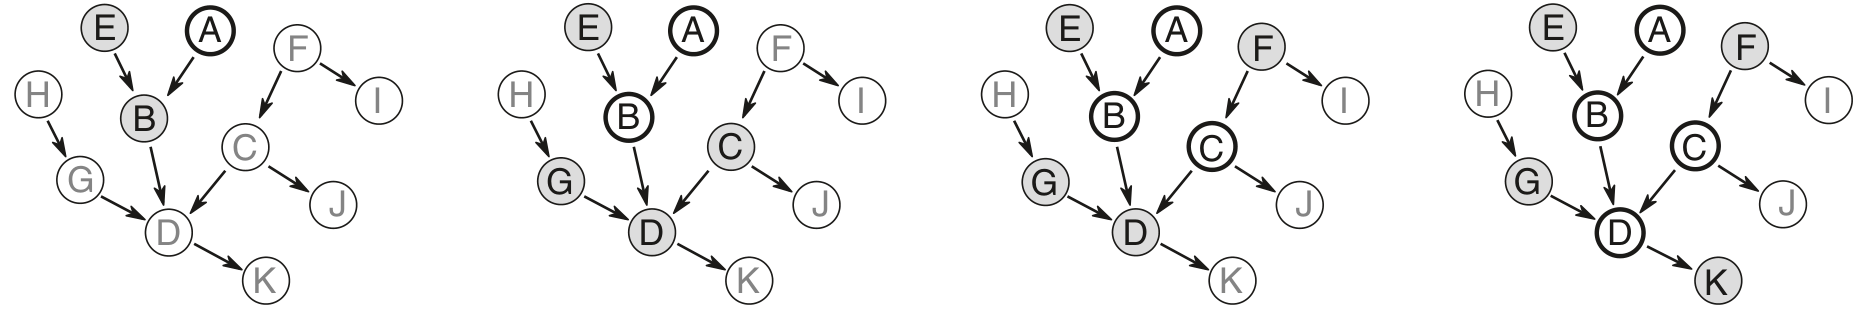
\includegraphics[scale=0.27]{../assets/greedy_mutex.png}
        
        \caption{Greedy expansion of $\{A\}$ (left to right).}
    \end{figure}
\end{example}

The \textit{proximity} $\delta(M)$ is utilized in line 2 of the algorithm to define the set of potential candidates that could expand $M$. Indeed, the goal of \textcite{mutex} is to identify mutually exclusive altered groups, where members share a \textbf{common downstream signaling target}. They state that this strategy narrows the search space to areas with a higher concentration of true positives. While it may slightly reduce \href{https://en.wikipedia.org/wiki/Precision_and_recall}{recall}, it also lessens the loss of statistical power associated with \href{https://en.wikipedia.org/wiki/Multiple_comparisons_problem}{multiple hypothesis testing}. Additionally, this approach provides an initial explanation for the observed mutual exclusivity, i.e. \textit{through a shared effect on a downstream gene}.

Another aspect to discuss is the \textit{null distribution} of a given gene $g \in M$, which represents $g$'s distribution under $H_0$ (defined in \cref{H_0}), denoted as $\mathcal N_g$ in the algorithm. Given a gene $g \in M$, \textcite{mutex} estimate $g$'s null distribution through a procedure that approximately involves the following steps:

\begin{enumerate}
    \item \textit{initialization}: define $\mathcal N_g$ as an empty list;
    \item \textit{iteration}: for $i = 1, \ldots, i_\mathrm{max}$ derive $\mathcal N_g \texttt{[}i\texttt{]}$ as follows:

        \begin{enumerate}
            \item randomly permute $g$'s alterations --- i.e., permute $g$'s column in $A$ randomly;
            \item let $M_g := \texttt{greedyMutex}(g, k_\mathrm{max}, G, A, \texttt{false})$;
            \item let $\mathcal P_g := \texttt{pValues}(M_g, A)$;
            \item let $\mathcal N_g \texttt{[}i\texttt{]} := \mathcal P_g\texttt{[}g\texttt{]}$.
        \end{enumerate}
\end{enumerate}

This is a \textit{sketch} of the complete procedure, and the omitted details extend well beyond the scope of this discussion. The main conclusion from this algorithm is that $g$'s \textit{null distribution} is derived from its $p$-value (namely $\mathcal P_g\texttt{[}g\texttt{]}$), computed when its alterations are randomly permuted. This randomization aims to modify $\gamma(g, M_g)$, simulating a scenario in which $H_0$ holds true, i.e. alterations in $\Gamma(g)$ are independent from mutations in $\Gamma(M - \{g\})$. Note that $\mathcal P_g\texttt{[}g\texttt{]}$ is computed through the \texttt{greedyMutex} function, with \texttt{final} set to \texttt{false} to prevent infinite recursion and avoid recomputing the \textit{null distributions}. In the \texttt{expandGroup} procedure, it will be assumed that for any $g \in M$, $\mathcal N_g$ can be computed as described.

With these definitions established, the \texttt{expandGroup} algorithm can be explained in detail. Specifically, it can be broken down into the following sections:

\begin{enumerate}
    \item if $\texttt{final} = \texttt{true}$, fill $\mathcal N$ such that $$\forall g \in M \quad \mathcal N \texttt{[}g\texttt{]} = \mathcal N_g$$ where $\mathcal N_g$ is $g$'s \textit{null distribution}, based on $g$'s $p$-value computed on $M$;
    \item \textit{initialization}: let $m_s$ be $M$'s \textit{score} (refer to \cref{score_mutex});
    \item \textit{iteration}: for each candidate $c$ in $\delta(M)$, compute as follows:
        \begin{enumerate}
            \item if $\texttt{final} = \texttt{true}$, update $\mathcal N$ such that $$\forall g \in (M \cup \{c\}) \quad \mathcal N \texttt{[}g\texttt{]} = \mathcal N_g'$$ where $\mathcal N_g'$ is $g$'s \textit{null distribution}, based both on $g$'s $p$-value computed on $M \cup \{c\}$, and on $\mathcal N_g$;
            \item let $c_s$ be $(M \cup \{c\})$'s score;
            \item if $c_s$ improves \textit{both} the current best score, and $m_s$, update the current best score with $c_s$.
        \end{enumerate}
    \item if the best candidate $b$ could be determined, return $M \cup \{b\}$; otherwise, return $M$.
\end{enumerate}

Note that this procedure requires $c_s$ to improve \textit{both} the current best score and $M$'s base score, meaning that suboptimal solutions are not explored by the algorithm.

Finally, the last procedure, which computes the mutual exclusivity score of a given gene set, can be introduced. Although this score is a crucial part of the metric developed by \textcite{mutex} to assess mutual exclusivity within a gene set, this algorithm could not be introduced in the previous chapter because it relies on the \textit{null distribution} dictionary $\mathcal{N}$, defined in \cref{expand_group_mutex}, which in turn depends on the \textit{null distribution} estimation, based on \cref{greedy_mutex} (with $\texttt{final} = \texttt{false}$).

\begin{algorithm}[H]
    \caption{
        \textit{Scoring procedure}: given a gene set $M$, a mutation matrix $A$, a boolean variable \texttt{final}, and a \textit{null distribution} dictionary $\mathcal N$, the algorithm computes $M$'s mutual exclusivity score.
    }

        \label{score_mutex}
    \begin{algorithmic}[1]
        \Function{score}{$M$, $A$, \texttt{final}, $\mathcal N$}
            \State $\mathcal P := \texttt{pValues}(M, A)$
            \If{$\texttt{final}$} \Comment{initial $p$-values correction}
                \For{$g \in M$}
                    % \State $c := 0$
                    \State $\mathcal N_g := \mathcal N\texttt{[}g\texttt{]}$
                    \State $c := \abs{\{i \mid \mathcal N_g\texttt{[}i\texttt{]} \le \mathcal P \texttt{[}g\texttt{]}\}}$
                    % \For{$i \in [1, \mathcal N_g.\texttt{len}()]$}
                    %     \If{$\mathcal N_g\texttt{[}i\texttt{]} \le \mathcal P\texttt{[}g\texttt{]}$}
                    %         \State $c \texttt{ += } 1$
                    %     \EndIf
                    % \EndFor
                    \State $\mathcal P\texttt{[}g\texttt{]} := \max\rbk{\mathcal P\texttt{[}g\texttt{]}, \dfrac{c}{\mathcal N_g.\texttt{len}()}}$
                \EndFor
            \EndIf
            \State \textbf{return} $\max_{g \in M}{\mathcal P\texttt{[}g\texttt{]}}$ \Comment{the \textit{least} significant is the \textit{largest}}
        \EndFunction
    \end{algorithmic}
\end{algorithm}

First, the algorithm evaluates $\mathcal P$, the $p$-value dictionary; then, if $\texttt{final} = \texttt{true}$, $\mathcal P$ is corrected for \textit{multiple hypothesis testing}. Finally, the largest value in $\mathcal P$ is returned. Note that both in line 7 and line 10, the largest value is chosen: this is because the \textit{larger} the $p$-value, the \textit{less significant} it is. Therefore, in line 7, the focus is on being as cautious as possible, while in line 10, the aim is to ensure that each member of $M$ contributes to the pattern. Lastly, the boolean variable \texttt{final} ensures that, during the evaluation of the \textit{null distributions}, the scores being used remain uncorrected.

The complete algorithm works by calling \texttt{greedyMutex} for each possible $g \in \mathcal G$ with \texttt{final} set to \texttt{true}, and then comparing the resulting sets. Finally, these sets may optionally undergo an \href{https://en.wikipedia.org/wiki/False_discovery_rate}{FDR} control procedure, which lies outside the scope of this work. Note that many details from the \href{https://github.com/PathwayAndDataAnalysis/mutex}{original code} have been removed for brevity, in each described algorithm.

\subsection{Results}

\textcite{mutex} applied their algorithm to identify mutual exclusion patterns in mutation and copy number profiles from multiple TCGA studies. The gene network they employed was cropped to the \textit{proximity} of significantly mutated genes (derived from MutSig \cite{mutsig}) and significantly altered genes (provided by GISTIC \cite{gistic}). Lastly, to reduce noise, genes with low alteration rates were filtered out in each study, and groups of up to 5 genes were examined.

They identified a total of 199 genes in their results, with 31 appearing in at least two studies. Notably, TP53 was the most recurrent gene, followed by well-known tumor suppressors and oncogenes such as PTEN, KRAS, and MYC. Among less recognized genes, \href{https://www.ncbi.nlm.nih.gov/gene/84033}{OBSCN} and \href{https://www.ncbi.nlm.nih.gov/gene/8289}{ARID1A} are highlighted for their potential roles in cancer --- the latter has previously been shown to act as a tumor suppressor in \href{https://en.wikipedia.org/wiki/Gastrointestinal_cancer}{gastrointestinal cancers} (GI). The most frequent common targets among the result groups include PIK3R1, HRAS, BRAF, MYC, RAC1, and \href{https://www.ncbi.nlm.nih.gov/gene/389}{RHOC}, with mutually exclusive alterations observed upstream of RHOC in five datasets. Although RHOC alterations are infrequent in TCGA samples, its overexpression is associated with cancer cell metastasis, suggesting that its activation may represent a significant downstream effect of driver alterations.

To assess the novelty of the findings, \textcite{mutex} examined co-citations of the recurrent genes with the term \curlyquotes{cancer}, using CoCiter. The last 10 genes on the list had fewer than 25 co-citations, indicating they are not well-established cancer drivers. However, further investigation revealed that 5 of these genes --- \href{https://www.ncbi.nlm.nih.gov/gene/8295}{TRRAP}, OBSCN, \href{https://www.ncbi.nlm.nih.gov/gene/6016}{RIT1}, \href{https://www.ncbi.nlm.nih.gov/gene/116986}{AGAP2}, and \href{https://www.ncbi.nlm.nih.gov/gene/6097}{RORC} --- contain so called \textit{mutation hotspots}. Mutation hotspots are DNA segments particularly prone to genetic alterations \cite{mutation_hotspot}, and are considered indicators of driver mutations, as changes in different regions of a driver gene can confer varying levels of selective advantage to a cancer cell --- passenger mutations are typically randomly distributed \cite{mutex}. Among the remaining 5 genes, the gene pair (\href{https://www.ncbi.nlm.nih.gov/gene/29956}{CERS2}, \href{https://www.ncbi.nlm.nih.gov/gene/23385}{NCSTN}) showed copy number alterations in the results.

Additionally, \textcite{mutex} compared the performance of their method with several previously published studies, including Dendrix \cite{dendrix}, MDPFinder \cite{mdpfinder}, and Multi-Dendrix \cite{multi-dendrix}. They derived a large dataset from breast cancer data in \href{https://www.cbioportal.org/}{cBioPortal}, which included 830 genes with an alteration rate of at least 3\% across 958 samples. This dataset was constructed through several steps aimed at randomizing gene alterations while preserving alteration ratios. Mutex outperformed the other methods, significantly improving the \href{https://en.wikipedia.org/wiki/Receiver_operating_characteristic}{receiver operating characteristic} (ROC) curves; notably, a modified version of Mutex that \textit{did not} use signaling networks showed decreased performance, highlighting the advantages of incorporating pathway information. In contrast, Dendrix, MDPFinder, and Multi-Dendrix performed poorly due to their reliance on the same weight function $W(M)$, which favors noise over signal. Moreover, other methods' generative models also struggled because they assumed equal alteration chances among group members. Mutex demonstrated improved scoring criteria and efficiency, exhibiting strong scalability in terms of memory and runtime, comparable to MDPFinder, and significantly more efficient than Dendrix and similar algorithms.

In conclusion, the greedy algorithm developed by \textcite{mutex} identified known mutually exclusive driver pathways, and highlighted potential roles for lesser-known genes, namely OBSCN, ARID1A and RHOC.

The following section will outline the different versions of the clustering algorithm, anticipated in the previous chapter.

\section{$\mathrm{C}^3$}

\subsection{Multiple versions}

In the final section of the previous chapter (namely, \cref{c3_chap2}), it was mentioned that \textcite{c3} developed multiple versions of their clustering algorithm; these variants will be explored in detail in the following paragraphs. In particular, they defined three methods for assigning weights to the edges of their gene graph $G$, to perform their vertex clustering algorithm, called $\mathrm{C}^3$ (\textit{knowledge-based} \cite{survey}):

\begin{enumerate}
    \item \textbf{ME-CO}, where $w^-$ depends on \textit{mutual exclusivity} and $w^+$ depends on \textit{coverage};
    \item \textbf{NI-ME-CO}, where $w^-$ depends on \textit{mutual exclusivity} and $w^+$ depends on \textit{coverage} and \textit{network information};
    \item \textbf{EX-ME-CO}, where $w^-$ depends on \textit{mutual exclusivity} and $w^+$ depends on \textit{coverage}, and \textit{expression data}.
\end{enumerate}

Note that $w^-$ depends solely on the mutual exclusivity component in each version of the algorithm, whereas the value of $w^+$ depends on the chosen algorithm variant. The following section will introduce the standard version of $\mathrm{C}^3$.

\subsection{The standard version}

The initial version of their clustering algorithm is the standard one, which considers only \textbf{mutual exclusivity} and \textbf{coverage}, and it is described below.

\begin{definition}[ME-CO]
    In the \textbf{ME-CO} version of the algorithm, the following definitions apply:

    \begin{equation}
        \forall u, v \in V(G) \quad w_{uv}^- := w^-_{uv}(\mathrm e)
    \end{equation}

    \begin{equation}
        \forall u, v \in V(G) \quad w_{uv}^+ := w^+_{uv}(\mathrm c)
    \end{equation}
\end{definition}

The definitions for $w_{uv}^-(\mathrm e)$ and $w_{uv}^+(\mathrm c)$ are provided in \cref{me_comp} and \cref{co_comp} respectively.

Note that in each variation discussed, optional rescaling is applied to ensure that the weight formulas satisfy additional constraints required later in the algorithm, though the specifics are beyond the scope of this analysis.

While this version of the algorithm does not include any external data, the variant outlined in the next section incorporates additional supplementary information into the weights.

\subsection{Integrating network information} \label{network_info}

Pan-cancer studies, as reported in multiple papers, have demonstrated a significant relationship between network topology and the distribution patterns of cancer drivers. Specifically, the impact of deleterious mutations on the phenotype can be mitigated by certain configurations of the corresponding protein complexes, while other arrangements can amplify their effect. For example, most variants found in healthy individuals tend to be located at the periphery of the interactome, where they do not affect network connectivity. In contrast, cancer-driver somatic mutations are more likely to occur in central, internal regions of the interactome and within highly integrated components \cite{c3}. This suggests that network topology significantly influences the impact of cancer driver mutations, and to assess the implications for cancer development, \textcite{c3} analyzed network distances between driver variants to identify patterns.

To precisely quantify the network distances between driver variants, \textcite{c3} computed the pairwise network distances between genes within a large pathway, comprising 8726 genes, by using an implementation of the standard \href{https://en.wikipedia.org/wiki/Dijkstra%27s_algorithm}{Dijkstra algorithm}. To reduce the computational cost of running Dijkstra's algorithm $O\rbk{8726^2}$ times, 1000 pairs were randomly selected for this test. Using the most comprehensive known driver list from the Cancer Gene Census (CGC) \cite{cgc}, the same distances were calculated for driver genes, this time for all gene pairs. The resulting distribution of shortest paths is shown in \cref{frequency_c3} \cite{c3}, revealing that the average shortest distance between drivers is \textit{significantly smaller} than that between two randomly selected genes.

\begin{figure}[H]
    \centering
    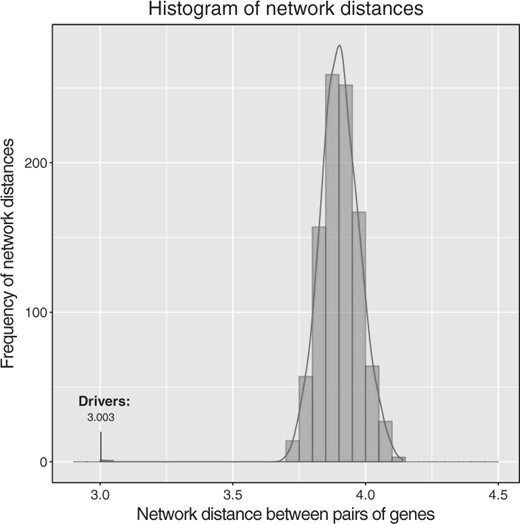
\includegraphics[scale=0.6]{../assets/frequency_c3.jpeg}
    
    \caption{Distribution of distances between genes in the network.} \label{frequency_c3}
\end{figure}

These findings indicate that network distance and connectivity information should be considered when identifying potential driver mutations. This can be achieved by adjusting the positive weight of edges connecting two genes: specifically, if both endpoint genes are drivers, they should be sufficiently central within a given pathway, close to other known drivers, or to each other.

Hence, from the KEGG \cite{kegg} database, \textcite{c3} built an undirected graph $G'$, where each vertex represents a gene and the edges describe interactions between them --- note that $\abs{V(G)} = \abs{V \left(G' \right)} = n$. For each vertex $u \in V \left(G' \right)$, let $\mathscr{N}(u)$ denote the set of $u$'s neighbors, and let $\mathscr{N}'(u) := \mathscr{N}(u) \cup \{u\}$. Also, let

\begin{equation}
    f(u, v) := \dfrac{\abs{\mathscr{N}'(u) \cap \mathscr{N}'(v)}}{\abs{\mathscr{N}'(u) \cup \mathscr{N}'(v)}}
\end{equation}

which is referred to as the \href{https://en.wikipedia.org/wiki/Jaccard_index}{Jaccard similarity coefficient}; a large value of $f(u, v)$ indicates that $u$ and $v$ are well connected in $G'$ and are likely involved in the same pathway, suggesting that they should be clustered together. Furthermore, let

\begin{equation}
    \mathscr{F} := \{f(u, v) \mid u, v \in V\rbk{G'}\}
\end{equation}

and let $T'(J')$ be the $J'$-th percentile of the values in $\mathscr F$.

The network information component of the positive weights is described below.

\begin{definition}[Network information component]
    The \textbf{network information component} is defined as follows: $$w_{uv}^+(\mathrm n) := \soe{ll}{1 & f(u, v) > T'(J') \\ \dfrac{f(u, v)}{T'(J')} & f(u, v) \le T'(J')}$$
\end{definition}

Finally, the version of $\mathrm{C}^3$ that incorporates the network information is defined as follows.

\begin{definition}[NI-ME-CO]
    The \textbf{NI-ME-CO} version of the algorithm is defined by the following equations:

    \begin{equation}
        \forall u, v \in V(G) \quad w_{uv}^- := w_{uv}^-(\mathrm e)
    \end{equation}

    \begin{equation}
        \forall u, v \in V(G) \quad w_{uv}^+ := w_1 w_{uv}^+(\mathrm c) + w_2 w_{uv}^+(\mathrm n)
    \end{equation}

    where $w_1, w_2 \ge 0$ and $w_1 + w_2 = 1$.
\end{definition}

The next section will describe a third variant, that incorporates gene expression data instead of network information.

\subsection{Integrating expression data}

Another valuable type of data that could be integrated into the positive weights for clustering is \textbf{gene expression data}. This is based on the assumption that co-expressed genes are likely to be involved in the same function or cancer pathway. Therefore, genes with strong positive or negative co-expression should be clustered together. The following paragrpahs will describe how \textcite{c3} include expression data into $w^+$.

Given a vertex $u \in V(G)$, let $\mathrm {\mathbf z(u)}$ be the vector of the time-evolving expression values of $u$ \todo{la prima volta che lessi questo paper non trovai niente sul dove presero queste informazioni, e tutt'ora non mi pare che lo menzionino da nessuna parte; scrivono solo che le informazioni le prendono dal TCGA e dal KEGG, suppongo a questo punto che queste info siano ottenibili dal TCGA ma dovrei controllare manualmente}. Thus, let

\begin{equation}
    g(u, v) := \dfrac{\abs{\abk{\mathrm{\mathbf z(u)}, \mathrm{\mathbf z(v)}}}}{\abs{\abs{\mathrm{\mathbf z(u)}}} \abs{\abs{\mathrm{\mathbf z(v)}}}}
\end{equation}

where $\abk{\mathrm{\mathbf a}, \mathrm{\mathbf b}}$ denotes the inner product of the vectors $\mathrm{\mathbf a}$ and $\mathrm{\mathbf b}$, while $\abs{\abs{\mathrm{\mathbf a}}}$ stands for its $L^2$ norm. This equation is known as the \href{https://en.wikipedia.org/wiki/Cosine_similarity}{cosine similarity}, since the ratio that defines $g(u, v)$ is equal to the cosine of the angle between $\mathrm {\mathbf z(u)}$ and $\mathrm {\mathbf z(v)}$ --- the only difference being the absolute value in the numerator, to capture both positive and negative correlations. A large value of $g(u, v)$ suggests that the expression vectors of $u$ and $v$ are highly correlated, hence they should be clustered together. Note that $$\forall u, v \in V(G) \quad 0 \le g(u, v) \le 1$$ Moreover, let

\begin{equation}
    \mathscr G := \{g(u, v) \mid u, v \in V(G)\}
\end{equation}

and let $T''(J'')$ be the $J''$-th percentile of the values in $\mathscr G$.

Hence, the gene expression component of the positive weights can be defined as follows.

\begin{definition}[Expression data component]
    The \textbf{expression data component} is defined as follows: $$w_{uv}^+(\mathrm x) := \soe{ll}{1 & g(u, v) > T''(J'') \\ \dfrac{g(u, v)}{T''(J'')} & g(u, v) \le T''(J'')}$$
\end{definition}

Lastly, the third variant of $\mathrm{C}^3$ is described below.

\begin{definition}[EX-ME-CO]
    The \textbf{EX-ME-CO} version of the algorithm is defined by the following equations:

    \begin{equation}
        \forall u, v \in V(G) \quad w_{uv}^- := w_{uv}^-(\mathrm e)
    \end{equation}

    \begin{equation}
        \forall w_{uv}^+ := w_1 w_{uv}^+(\mathrm c) + w_2 w_{uv}^+(\mathrm x)
    \end{equation}

    where $w_1, w_2 \ge 0$ and $w_1 + w_2 = 1$.
\end{definition}

\subsection{Other versions}

\textcite{c3} also mention that other combinations can be used, with appropriate adjustments to the weights, such as the following version, which will be referred to as NI-EX-ME-CO in this work.

\begin{definition}[NI-EX-ME-CO]
    The \textbf{NI-EX-ME-CO} version of the algorithm is defined by the following equations:

    \begin{equation}
        \forall u, v \in V(G) \quad w_{uv}^- := w_{uv}^-(\mathrm e)
    \end{equation}

    \begin{equation}
        \forall w_{uv}^+ := w_1 w_{uv}^+(\mathrm c) + w_2 w_{uv}^+(\mathrm n) + w_3 w_{uv}^+(\mathrm x)
    \end{equation}

    where $w_1, w_2, w_3 \ge 0$ and $w_1 + w_2 + w_3 = 1$.
\end{definition}

The previous sections outlined the definition of the weights for the edges in the gene graph $G$; instead, the following ones will explain how $\mathrm{C}^3$ operates.

\subsection{The clustering ILP} \label{the_clustering_ilp}

\textcite{c3} opted to use an ILP approach to formulate the clustering algorithm, utilizing the weights defined in the previous sections.

Note that the classical formulation of correlation clustering does not impose any restrictions on cluster sizes. However, most driver identification methods inherently include cluster size limits, as they directly affect the computational complexity of the algorithms --- many even fail to operate beyond a certain size. Another reason for imposing a cluster size limit is the expectation that driver genes of specific cancer types will be grouped together, and recent findings indicate that only a small number of drivers are typically present in any given cancer type. Thus, if clusters are too large, they may include drivers from multiple cancer types, hiding this separation of the drivers. Furthermore, introducing cluster size constraints helps to avoid the formation of non-informative \textit{giant clusters} or \textit{singleton clusters} \cite{c3}.

Therefore, \textcite{c3} introduce a cluster size constraint by assuming that all clusters are of size $k$ at most; clearly, setting $k$ equal to the total number of vertices effectively removes this constraint, allowing flexibility in cluster size selection.

The ILP of $\mathrm{C}^3$ is defined as follows.

\begin{definition}[$\mathrm{C}^3$'s ILP] \label{c3_ilp}
    The \textbf{$\mathrm{C}^3$ algorithm} can be defined by the following ILP:

    \begin{equation} \label{c3_first}
        \mathrm{minimize} \sum_{e \in E(G)} (w_e^+x_e + w_e^-(1 - x_e)),
    \end{equation}

    \begin{equation} \label{c3_second}
        \mathrm{subject \ to \ } x_{uv} \le x_{uz} + x_{zv}, \quad u, v, z \in V(G) \mathrm{\ distinct},
    \end{equation}

    \begin{equation} \label{c3_third}
        \sum_{v \in V(G) \atop u \neq v} (1 - x_{uv}) \le k, \quad u \in V(G),
    \end{equation}

    \begin{equation} \label{c3_fourth}
        x_e \in \{0, 1\}, \quad e \in E(G).
    \end{equation}
\end{definition}

In this formulation, the variables $x_e$ allow to describe any clustering of the vertices of $G$, since $x_e \in \{0, 1\}$ for each $e \in E(G)$.

Note that \cref{c3_first} aligns with the definition provided in \cref{c3_chap2}, as $x_{uv} = 1$ implies that $u$ and $v$ should belong to different clusters, while $x_{uv} = 0$ implies that the two vertices should be placed into the same cluster.

Furthermore, \cref{c3_third} states that for a fixed vertex $u \in V(G)$, the number of variables $x_{uv}$ equal to 0, for any $v \in \mathcal N(u)$, must not exceed $k$ --- which is the clustering size constraint previously discussed.

Lastly, \cref{c3_second} is the \href{https://en.wikipedia.org/wiki/Triangle_inequality}{triangle inequality}, which ensures that if $u$ and $z$ are placed in the same cluster, and $z$ and $v$ are also placed in the same cluster, then $u$ and $v$ will be clustered together. This means that \textit{belonging to the same cluster is a transitive property}, since $$\soe{l}{x_{uz} = 0 \\ x_{zv} = 0 \\ x_{uv} \le x_{uz} + x_{zv}} \implies x_{uv} = 0$$

The next section will illustrate a relaxation of this ILP.

\subsection{The rounding procedure}

Since solving binary ILPs is \NPComplete \cite{karp}, \textcite{c3} relax the problem by changing \cref{c3_fourth} to an interval constraint $$0 \le x_e \le 1$$ leading to an LP program, the solution of which may be fractional. Hence, to obtain a valid clustering, the fractional solutions have to be rounded. Therefore, instead of solving the LP, they remove \cref{c3_third} from the linear program, and employ the following rounding procedure to round the fractional values.

\begin{algorithm}[H]
    \caption{
        \textit{Rounding procedure}: given a solution $\{x_e\}_{e \in E(G)}$ of the relaxed version of the ILP provided \cref{c3_ilp}, a rational value $\alpha$, and the maximum cluster size $k$, the algorithm rounds the solution to integer values.
    }

        \label{rounding_procedure}
    \begin{algorithmic}[1]
        \Function{roundingProcedure}{$G$, $\{x_e\}_{e \in E(G)}$, $\alpha$, $k$}
            \State $\mathcal C := \varnothing$ \Comment{the output set of clusters}
            \State $S := V(G)$
            \While{$S \neq \varnothing$}
                \State Choose an arbitrary $u \in S$ \Comment{this is the \textit{pivot vertex}}
                \State $T := \{w \in S - \{u\} \mid x_{uw} \le \alpha\}$ \Comment{$u$'s neighbors under $\alpha$'s threshold}
                \If{$\sum_{w \in T}{x_{uw}} \ge \frac{\alpha}{2}\abs{T}$}
                    \State $\mathcal C = \mathcal C \cup \{\{u\}\}$ \Comment{add a singleton cluster $\{u\}$}
                    \State $S = S - \{u\}$
                \ElsIf{$\abs{T} \le k$}
                    \State $\mathcal C = \mathcal C \cup \{\{u\} \cup T\}$ \Comment{add the cluster $(\{u\} \cup T)$}
                    \State $S = S - \rbk{\{u\} \cup T}$
                \Else
            \State Partition $T$ into $\{T_0', T_1, \ldots, T_p\}$, such that: \begin{itemize} \item[] \quad \quad \quad \quad $\sbullet \ \abs{T_0'} = k$ \item[] \quad \quad \quad \quad $\sbullet \ \abs{T_i} = k + 1$ for each $0 < i < p$ \item[] \quad \quad \quad \quad $\sbullet \ \abs{T_p} \le k + 1$ \end{itemize}
                    \State $T_0 := T_0' \cup \{u\}$ \Comment{$T_0$ has $k + 1$ elements}
                    \For{$i \in [0, p]$}
                        \State $\mathcal C = \mathcal C \cup \{T_i\}$ \Comment{add each partition as a cluster}
                    \EndFor
                    \State $S = S - \rbk{\{u\} \cup T}$
                \EndIf
            \EndWhile
            \State \textbf{return} $\mathcal C$
        \EndFunction
    \end{algorithmic}
\end{algorithm}

The algorithm can be summarized as follows:

\begin{enumerate}
    \item \textit{initialization}: let $\mathcal C := \varnothing$ and $S := V(G)$;
    \item \textit{iteration}: while $S \neq \varnothing$, compute as follows:
        \begin{enumerate}
            \item choose a \textit{pivot} vertex $u \in S$ arbitrarily;
            \item let $T$ be the set of $u$'s neighbors $w \in \mathcal N (u)$ such that $x_{uw}$ is at most $\alpha$;
            \item if $\frac{\alpha}{2} \abs{T}$ is at most $\sum_{w \in T}{x_{uv}}$, add $\{u\}$ to $\mathcal C$ as a \textit{singleton cluster}, and remove $u$ from $S$;
            \item otherwise, if $\abs{T}$ is at most $k$, add $\{u\} \cup T$ to $\mathcal C$ as a cluster, and remove it from $S$;
            \item otherwise, partition $T$ in multiple subsets, such that each subset contains $k + 1$ elements (technically, the last partition will contain only the remaining elements), and the first subset contains $u$; then, add each partition of $T$ as a separate cluster to $\mathcal C$, and remove every partition from $S$.
        \end{enumerate}
\end{enumerate}

The rationale behind the condition in line 7 can be elucidated by examining the meaning of $x_{uw}$: specifically, if $x_{uw}$ is close to 1, $u$ and $w$ are likely to be placed in different clusters, as previously described \cref{the_clustering_ilp}. Note that, if the sum $\sum_{w \in T}{x_{uw}}$ is greater than or equal to a value proportional to $\abs T$, it indicates that there are numerous edges $(u, w)$ for $w \in T$ with significantly high $x_{uw}$. Therefore, this suggests that $u$ should likely be placed in a cluster distinct from all its \textit{filtered} neighbors $T$.

In contrast, if this condition does not hold, it is probable that several variables indicate that $u$ should be clustered with some of its \textit{filtered} neighbors. Therefore, when this condition fails, and $\abs T \le k$, $u$ and $T$ are forced to form a cluster in line 11.

Lastly, if none of the preceding conditions are satisfied, it means that $u$ should not form a \textit{singleton cluster}, but the presence of numerous \textit{filtered} neighbors precludes the formation of a $T \cup \{u\}$ cluster. Therefore, line 14 partitions $T$ into smaller clusters of size $k + 1$.

As a final note, \textcite{c3} conducted an analysis to determine the optimal value for $\alpha$, which was found to be $\frac{2}{7}$, but the proof of this value is beyond the scope of this work.

Finally, the complete $\mathrm{C}^3$ algorithm that \textcite{c3} employed to obtain their results is described below.

\begin{definition}[$\mathrm{C}^3$] \label{c3_final}
    The \textbf{$\mathrm{C}^3$ algorithm} is defined as follows: first, the next ILP is solved

    \begin{equation}
        \mathrm{minimize} \sum_{e \in E(G)} (w_e^+x_e + w_e^-(1 - x_e)),
    \end{equation}

    \begin{equation}
        \mathrm{subject \ to \ } x_{uv} \le x_{uz} + x_{zv}, \quad u, v, z \in V(G) \mathrm{\ distinct},
    \end{equation}

    \begin{equation}
        0 \le x_e \le 1, \quad e \in E(G).
    \end{equation}

    and then the rounding procedure defined in \cref{rounding_procedure} is applied.
\end{definition}

\subsection{Results}

To perform a comparative analysis with an existing study, \textcite{c3} selected the CoMEt algorithm --- developed by \textcite{comet} --- for comparison, and the results of their analysis are detailed below. In particular, they ran both algorithms utilizing mutation and CNV data sourced from the TCGA \cite{tcga} database, specifically focusing on BRCA and GBM.

Both algorithms were tested on a high-memory server under identical conditions, except when CoMEt encountered memory errors at cluster size $k = 15$, allowing only $\mathrm{C}^3$ to be tested for that case. This highlights the computational flexibility of their algorithm, particularly in terms of adjusting both the cluster size $k$ and the number of clusters formed. In the benchmark \textcite{c3} focused on the following evaluation criteria:

\begin{itemize}
    \item to assess the \textit{mutual exclusivity} within a cluster, they evaluated the median pairwise exclusivity for each gene pair $(g_1, g_2)$ of the cluster, utilizing Fisher's exact test --- specifically, they used the same contingency table described in \cref{contingency}, but in their case $M = \{g_1, g_2\}$;
    \item to quantify the \textit{coverage} of a given cluster, they calculated the propotion of patients who exhibited at least one alteration in a gene of the cluster;
    \item as mentioned in \cref{network_info}, driver genes tend to cluster closer together within biological pathways compared to random gene selections; therefore, to identify potential cancer driver genes, they measured the shortest network distances between genes in the discovered clusters;
    \item lastly, to determine biological significance based on driver genes, they calculated the proportion of known drivers within the ten most mutually exclusive clusters, using a curated list of driver genes from the CGC \cite{cgc}.
\end{itemize}

When analyzing \textit{mutual exclusivity}, $\mathrm{C}^3$ demonstrated better performance, particularly for BRCA, where it produced more mutually exclusive clusters with lower $p$-values across most cluster sizes. Both methods found biologically significant clusters, but $\mathrm{C}^3$'s median exclusivity scores were generally stronger, except for cluster size $k = 10$. For GBM, the results were less pronounced due to the smaller dataset, but $\mathrm{C}^3$ still outperformed CoMEt in overall mutual exclusivity.

Regarding \textit{coverage}, CoMEt was superior in GBM, where it achieved a higher median coverage of 0.696 compared to $\mathrm{C}^3$'s 0.632. For BRCA, however, both algorithms performed similarly, with no significant difference in coverage. The choice of weights in $\mathrm{C}^3$, which prioritized mutual exclusivity over coverage, likely contributed to its lower coverage performance.

Moreover, in the \textit{pairwise distance} analysis of clustered genes, $\mathrm{C}^3$ and CoMEt performed similarly for BRCA, but $\mathrm{C}^3$ showed a statistically significant improvement in GBM, with smaller average distances between genes in clusters. This indicates that $\mathrm{C}^3$ tends to favor more tightly related clusters in cancer pathways, particularly for GBM.

Lastly, in terms of \textit{driver identification}, $\mathrm{C}^3$ outperformed CoMEt across all cluster sizes. For BRCA, $\mathrm{C}^3$ achieved a median driver proportion of 0.160 in the top ten clusters, while CoMEt reached 0.117. A similar trend was observed for GBM, where $\mathrm{C}^3$ found a median driver proportion of 0.170 compared to CoMEt's 0.120.

In addition to this analysis, \textcite{c3} tested $\mathrm{C}^3$'s ability to identify clusters of genes that may represent novel candidate cancer drivers, focusing on those with biologically significant interactions and high mutual exclusivity and coverage. The analysis particularly emphasized large cluster sizes, which have not been extensively reported in the literature.

For BRCA, a notable cluster included several potential driver genes such as PTEN, \href{https://www.ncbi.nlm.nih.gov/gene/10075}{HUWE1}, \href{https://www.ncbi.nlm.nih.gov/gene/26047}{CNTNAP2}, \href{https://www.ncbi.nlm.nih.gov/gene/2895}{GRID2}, \href{https://www.ncbi.nlm.nih.gov/gene/774}{CACNA1B}, \href{https://www.ncbi.nlm.nih.gov/gene/57105}{CYSLTR2}, and \href{https://www.ncbi.nlm.nih.gov/gene/4619}{MYH1}, with a mutual exclusivity $p$-value of 0.0084. This cluster is primarily influenced by mutations in PTEN and HUWE1, with PTEN being a well-known tumor suppressor gene, and the other genes in the cluster are also potential drivers, with roles in apoptosis, DNA repair, and cell signaling. The tightly interconnected nature of these genes suggests they may collectively define a new driver pathway, supported by the presence of high-impact common drivers like TP53 and MYC, which are critical in cancer pathways such as apoptosis and DNA repair.

In the GBM analysis, a cluster of size 10 genes was identified, containing four known drivers (\href{https://www.ncbi.nlm.nih.gov/gene/2735}{GLI1}, \href{https://www.ncbi.nlm.nih.gov/gene/7472}{WNT2}, BRAF, \href{https://www.ncbi.nlm.nih.gov/gene/7472}{PLCG1}) alongside several potential drivers. Notably, this cluster showed a mutual exclusivity $p$-value of 0.0901, which is relatively low for GBM. The genes in this cluster are involved in various pathways related to cell growth, apoptosis, and DNA repair, with six of the ten genes forming a compact network community. For instance, GLI1 and GLI2 are key \href{https://en.wikipedia.org/wiki/Hedgehog_signaling_pathway}{hedgehog signaling} genes linked to glioblastoma, playing crucial roles in cell differentiation and stem cell self-renewal.

In conclusion, $\mathrm{C}^3$ outperformed CoMEt in mutual exclusivity, driver gene identification, and cluster tightness, particularly for BRCA. Although CoMEt had better coverage in GBM, $\mathrm{C}^3$ identified more biologically significant clusters and handled larger cluster sizes without errors, making it a more robust tool for cancer research.

\cleardoublepage

% \chapter{Discussion} \label{chap:discussion}

placeholder. \todo{introduction to the chapter}

\section{Dendrix}

\subsection{The deterministic formalization}

\textcite{dendrix} provided one of the first mathematical formalizations of the phenomena of mutual exclusivity and coverage, in the context of gene mutations. Specifically, the definitions introduced offer a very intuitive approach to formalizing these biological concepts:

\begin{itemize}
    \item the coverage of a gene is defined as the set of patients exhibiting a mutation of the gene, equivalent to the number of 1s in its column of the mutation matrix;
    \item a set of genes is defined to be mutually exclusive if no patient has more than one mutated gene in the set, i.e. no row of the set's associated matrix has more than 1 one;
    \item the coverage of a gene set is the set of patients with at least one mutation in the set;
    \item the coverage overlap of a gene set is the count of patients who possess more than one mutation within the gene set;
    \item the weight of a gene set is calculated as the difference between the coverage of the gene set and its coverage overlap.
\end{itemize}

Consequently, a higher weight for a gene set indicates both greater coverage and mutual exclusivity among its genes. The weight formula suggests that the optimal gene set, i.e. the one that maximazes its weight, is the one where the associated matrix has a high number of rows with at least one 1, and a minimal number of rows with more than one 1.

In my view, this metric stands out as the most elegant among those discussed in this work: it not only provides a clear and intuitive measure, but also offers a simple and straightforward formula. While this approach may seem to oversimplify the challenge of identifying driver pathways --- given that mutual exclusivity alone does not cover all aspects of pathway analysis --- it remains a highly regarded deterministic formalization, and numerous studies (some of which are discussed in this work) agree that this metric represents the most refined approach to date.

% therefore, the higher the weight of a gene set, the higher its coverage and the mutual exclsuivity of its genes. looking at the formula, clearly the gene set that maximizes its weight is the one in which its associated matrix has at least 1 one in most rows, and the least possible amount of rows with more than 1 one in them.

% i personally think that this metric is the best one out of all the studies reported in this work. it is the one that makes sense the most, and i think is a rather elegant formula, for its simplicity. speaking of which, it may seems this equation oversimplifies the problem of finding driver pathways, as it's always the case, the assumption of mutual exclusivity is not the end of the story, and surely there is more that we still don't know. nevertheless, multiple studies (some of which are discussed in this work) agree that this metric is the best deterministic formalization yet.

\subsection{The approach}

as proved in \cref{todo}, finding the optimal set is np-complete. in order to solve the MWSP, they provide an approach that may not seem the most straightforward, since the very definition of the problem resambles an \href{https://en.wikipedia.org/wiki/Optimization_problem}{optimization problem}, but the MCMC algorithm they employ effectively finds gene groups known to be involved in cancer proliferation. it would be intresting to conduct a further analysis, comparing the MCMC method with a random search approach

\begin{enumerate}
    \item \textit{initialization}: given the set of all genes $\mathcal G$, choose an arbitrary subset $M_0 \subseteq \mathcal G$ ok $k$ genes;
    \item \textit{iteration}: for $t = 1, 2, \ldots$ derive $M_{t + 1}$ from $M_t$ as follows:

    \begin{enumerate}
        \item define $W \subseteq \mathcal G$ and $V \subseteq M_t$ randomly;
        \item choose $\displaystyle (\hat w, \hat v) \in \argmax_{(w, v) \in W \times V}{W\rbk{\rbk{M_t - \{v\}} \cup \{w\}}}$;
        \item set $M_{t + 1} := \rbk{M_t - \{\hat v\}} \cup \{\hat w\}$.
    \end{enumerate}
\end{enumerate}

at each step, this algorithm defines a predetermined amount of \textit{random adjustment}, and the one that increases the weight the most is choosen as the base set for the next iteration. it would be interesting to test how this approach performs on real data, and whether the MCMC outperforms it, especially when the data is under the GIM model

\section{Multi-Dendrix}

\subsection{An ILP for the MWSP}

also, as previously mentioned by the authors of multiple of the paper discussed, the set $M$ that maximizes $W(M)$ may not be a real driver pathway in real life. in fact, i too believe that exact solutions to the associated MWSP problem may not be correct, since 

\cleardoublepage

% 
\chapter{Parity in black-box \textsf{TFNP}} \label{chap:parity-tfnp}


\cleardoublepage


% ================== Notes ==================
% 

\chapter{Notes} \label{chap:notes}

Tree-like resolutions for an unsatisfiable CNF formula are strictly connected to the decision trees that solve its associated search problem. In particular, it can be proven that the smallest tree-like refutation has the exact same structure of the smallest decision tree. 

\begin{lemma} \label{lem:treeres_dt}
    \cite{treelike_res_size}
    Let $F$ be an unsatisfiable CNF formula. If there is a tree-like refutation of $F$ with structure $T$, there also exists a decision tree with structure $T$ that solves $\mathrm{Search}(F)$
\end{lemma}

\begin{proof}
    We procede by induction on the size $s$ of the refutation of $F$.

    Let $F = C_1 \land \ldots \land C_m$. If $s = 1$, then the refutation is made up of only one step that ends with the empty clause, implying that $\exists i \in [m]$ such that $F = C_i = \bot$. Hence, $\mathrm{Search}(F)$ can be solved by the decision tree made of only one vertex labeled with $i$.

    We now assume that every formula with a tree-like refutation with a structure of size $s$ there exists a decision tree with the same structure that solves the search problem associated with the formula.

    Suppose now that the size $s$ of the refutation is bigger than 1. Let $x$ be the last variable resolved by the refutation and let $T_0$ and $T_1$ be the subtrees of $T$ such that $x$ is the root of $T_0$ and $\lnot{x}$ is the root of $T_1$.

    Consider now the formulas $F{\upharpoonright_{x=0}}$ and $F{\upharpoonright_{x=1}}$, respectively corresponding the formula $F$ with the value $0$ or $1$ assigned to $x$. It's easy to see that the subtrees $T_0$ and $T_1$ are valid refutations of the formulas $F{\upharpoonright_{x=0}}$ and $F{\upharpoonright_{x=1}}$: if $b = 0$, then $x$ evaluates to $0$, otherwise if $b = 1$ then $\lnot{x}$ evaluates to 0.

    Since $T_0$ and $T_1$ have size $s-1$, by inductive hypothesis there exist two decision tree with structure $T_0$ and $T_1$ that solve $\mathrm{Search}(F{\upharpoonright_{x=0}})$ and $\mathrm{Search}(F{\upharpoonright_{x=1}})$.

    Finally, the search problem $\mathrm{Search}(F)$ can be solved by the decision tree that queries $x$ and proceeds with the decision tree $T_b$ based on the value $b \in \{0,1\}$ such that $x = b$.

\end{proof}

\begin{definition}
Given two rooted trees $T$ and $T'$, we say that $T$ is embeddable in $T'$ if there exists a mapping $f : V(T) \to V(T')$ such that, for any vertices $u,v \in V(T)$, if $u$ is a parent of $v$ in $T$ then $f(u)$ is an ancestor of $f(v)$ in $T'$.
\end{definition}

\begin{lemma} \label{lem:dt_treeres}
    \cite{treelike_res_size,search_problems_dt_model}
    Let $F$ be an unsatisfiable CNF formula. If there is a decision tree with structure $T$ that solves $\mathrm{Search}(F)$, there also exists a tree-like refutation of $F$ with structure $T'$ such that $T'$ is embeddable in $T$.
\end{lemma}

\begin{proof}

    The main idea is to associate inductively, starting from the leaves, a clause to each vertex of $T$ in order to transform $T$ in a tree-like refutation of $F$. In particular, each vertex $v$ gets associated to a clause $C(v)$ such that every input of the decision tree that reaches $v$ falsifies $C(v)$.

    Let $F = C_1 \land \ldots \land C_m$. For all $i \in [m]$, we associate the clause $C_i$ to the leaf of $T$ labeled with $i$. This constitutes our base case.

    Consider now a vertex $v$ that isn't a leaf. Let $x$ be the variable that labels $v$ and let $u_0, u_1$ be the vertices such that the edge $(v, u_0)$ is taken if $x = 0$ and the edge $(v, u_1)$ is taken if $x = 1$.  By induction, assume that $u_0$ and $u_1$ have already been associated with the clauses $C_0$ and $C_1$.

    By way of contradiction, suppose that $C_0$ contains the literal $\lnot{x}$. Then, since in a decision tree each variable can be queried only once in every path, there will always be an input with $x = 0$ that reaches $v$. Since $x = 0$ and since $C_0$ contains $\lnot{x}$, this input would satisfy $C_0$, contradicting the fact that $C_0$ was associated to $u_0$ in a way that it is falsified by every input.

    Thus, the only possibility is that $C_0$ can't contain the literal $\lnot{x}$. Similarly, we can show that $C_1$ can't contain the literal $x$. This leaves us with only two possibilities: either $C_0 = x \lor \alpha$ and $C_1 = \lnot{x} \lor \beta$ or one of $C_0, C_1$ doesn't contain $x, \lnot{x}$.

    In the first case, we can simply associate to $v$ the clause $C = \alpha \lor \beta$.  In the second case, we associate to $v$ the clause that doesn't contain $x, \lnot{x}$ (chose any of them if both clauses do not contain $x, \lnot{x}$).

    In particular, we notice that the first case directly emulates the resolution rule, while the second case essentially represent "redundant steps". By "skipping" these redundant steps, we can obtain a tree $T'$ that is embeddable in $T$ and that contains only nodes on which the first case was applied. Finally, it's easy to deduce that the root node of $T'$ will always be associated with the empty clause $\bot$, concluding that $T'$ is the structure of a tree-like refutation of $F$.

\end{proof}

\begin{theorem}
Let $F$ be an unsatisfiable CNF formula. The smallest tree-like refutation of $F$ has size $s$ and depth $d$ if and only if the smallest decision tree solving $\mathrm{Search}(F)$ has size $s$ and depth $d$.
\end{theorem}

\begin{proof}
    Let $s$ and $d$ be the size and depth of the smallest tree-like refutation of $F$. Likewise, let $x$ and $y$ be the size and depth of the smallest decision tree solving $\mathrm{Search}(F)$.

    Then, by \Cref{lem:treeres_dt}, we know that there exists a decision tree that solved $\mathrm{Search}(F)$ with the same structure of the smallest refutation. Let $\alpha$ and $\beta$ be the size and depth of this decision tree. It's easy to see that $s = \alpha \geq x$ and $d = \beta \geq y$.

    Viceversa, by \Cref{lem:dt_treeres}, we know that there exists a tree-like refutation of $F$ such that its structure is embeddable in the one of the smallest decision tree. Let $\gamma$ and $\beta$ be the size and depth of this tree-like refutation. Since the latter is embedded in the smallest decision tree, it's structure must be smaller or equal. Hence, it's easy to see that $x \geq \gamma \geq s$ and $y \geq \delta \geq d$. Thus, we can conclude that $s = x$ and $d = y$.

\end{proof}

\textbf{Note:} \cite{proofs_circuits_communication} says that this theorem should be generalizable to each tree and not only for the smallest trees (doubt this is true)

\newpage

\begin{figure}[H]
\centering

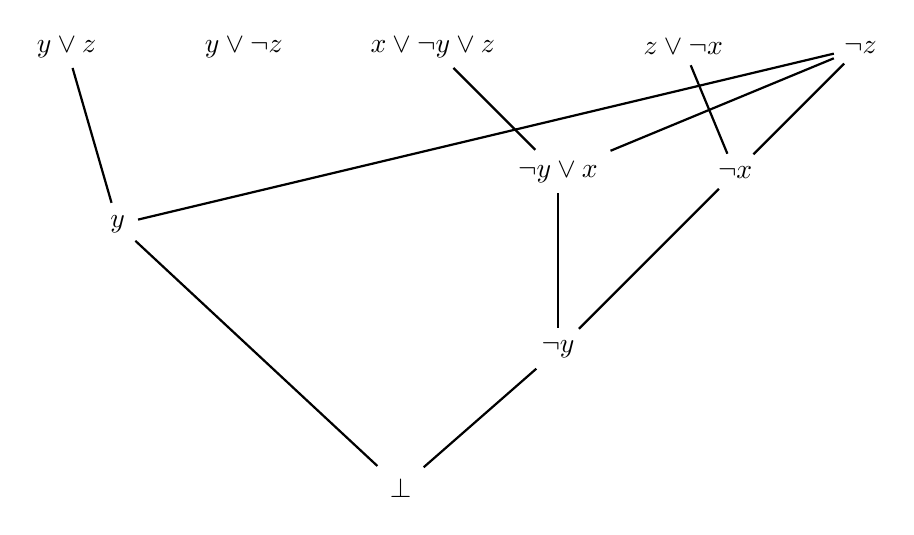
\begin{tikzpicture}[-,>=stealth,shorten >=1pt,auto,node distance=2.25cm, thick,main node/.style={scale=0.9,circle,draw,font=\sffamily\normalsize}]
    \node (1) []{$\bot$};
    
    \node (2) at ($(1)+(-2,1.75)$){};
    \node (3) at ($(1)+(2,1.75)$){$\lnot{y}$};

    \node (4) [above left of=2]{};
    \node (5) [above right of=2]{};

    \node (6) [above of=3]{$\lnot{y} \lor x$};
    \node (7) [right of=6]{$\lnot{x}$};
    
    \node (8) [above left of=6]{$x \lor \lnot{y} \lor z$};
    \node (9) [above right of=6]{$z \lor \lnot{x}$};

    \node (11) [right of=9]{$\lnot{z}$};
    \node (12) [above left of=2]{$y$};

    \node (14) at ($(8)+(-2.4,0)$){$y \lor \lnot{z}$};
    \node (15) [left of=14]{$y \lor z$};

    \path[every node/.style={font=\sffamily\small}]
        (15) edge (12)
        
        (6) edge (3)
        (7) edge (3)
        
        (8) edge (6)
        (11) edge (6)
        
        (9) edge (7)
        (11) edge (7)

        (11) edge (12)

        (12) edge (1)
        (3) edge (1)
    ;
\end{tikzpicture}

\caption{Dag-like refutation of the previous formula}
\end{figure}

\begin{figure}[H]
\centering

\begin{tikzpicture}[-,>=stealth,shorten >=1pt,auto,node distance=2.25cm, thick,main node/.style={scale=0.9,circle,draw,font=\sffamily\normalsize}]

    \node (1) []{$\bot$};
    
    \node (2) at ($(1)+(-2,1.75)$){$y$};
    \node (3) at ($(1)+(2,1.75)$){$\lnot{y}$};

    \node (4) [above left of=2]{};
    \node (5) [above right of=2]{};

    \node (6) [above of=3]{$\lnot{y} \lor z$};
    
    \node (8) [above left of=6]{$x \lor \lnot{y} \lor z$};
    \node (9) [above right of=6]{$z \lor \lnot{x}$};

    \node (11) [right of=9]{$\lnot{z}$};

    \node (14) at ($(8)+(-2.4,0)$){$y \lor \lnot{z}$};
    \node (15) [left of=14]{$y \lor z$};

    \path[every node/.style={font=\sffamily\small}]
        (14) edge (2)
        (15) edge (2)

        (8) edge (6)
        (9) edge (6)

        (6) edge (3)
        (11) edge (3)

        (2) edge (1)
        (3) edge (1)
    ;
\end{tikzpicture}

\caption{Tree-like refutation of the previous formula}
\end{figure}

\begin{figure}[H]
\centering

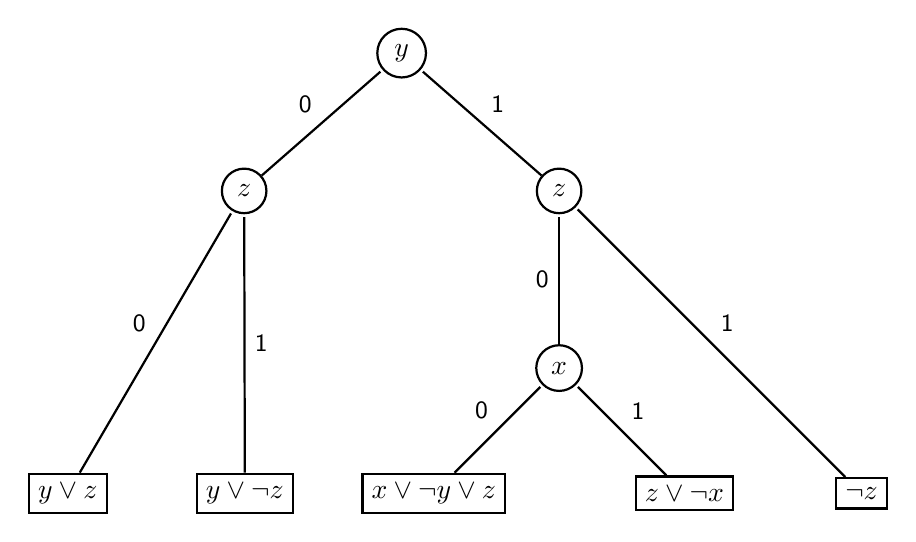
\begin{tikzpicture}[-,>=stealth,shorten >=1pt,auto,node distance=2.25cm, thick,main node/.style={scale=0.9,circle,draw,font=\sffamily\normalsize}]

    \node (1)[circle, draw]{$y$};
    
    \node (2) at ($(1)+(-2,-1.75)$) [circle, draw]{$z$};
    \node (3) at ($(1)+(2,-1.75)$) [circle, draw]{$z$};

    \node (4) [below left of=2]{};
    \node (5) [below right of=2]{};

    \node (6) [below of=3, circle, draw]{$x$};
    
    \node (8) [below left of=6, rectangle, draw]{$x \lor \lnot{y} \lor z$};
    \node (9) [below right of=6, rectangle, draw]{$z \lor \lnot{x}$};

    \node (11) [right of=9, rectangle, draw]{$\lnot{z}$};

    \node (14) at ($(8)+(-2.4,0)$) [rectangle, draw]{$y \lor \lnot{z}$};
    \node (15) [left of=14, rectangle, draw]{$y \lor z$};

    \path[every node/.style={font=\sffamily\small}]
        (14) edge [swap] node{1} (2)
        (15) edge node{0} (2)

        (8) edge node{0}(6)
        (9) edge node[swap]{1}(6)

        (6) edge node{0}(3)
        (11) edge [swap] node{1}(3)

        (2) edge node {0} (1)
        (3) edge node [swap] {1} (1)
    ;
\end{tikzpicture}

\caption{Decision tree for the previous formula}
\end{figure}


\section{The $\frac{1}{3}, \frac{2}{3}$ lemma}

\begin{definition}
    Given a tree $T$ and a node $v$, we denote as $T_v$ the subtree of $T$ having $v$ as its radix. 
\end{definition}

\begin{lemma}[Lewis' $\frac{1}{3}, \frac{2}{3}$ lemma \cite{1-3_2-3}]
    \label{13_23_lewis}
    If $T$ is a binary tree of size $s > 1$ then there is a node $v$ such that the subtree $T_v$ has size between $\floor{\frac{1}{3} s}$ and $\ceil{\frac{2}{3} s}$.
\end{lemma}

\begin{proof}
    Let $r$ be the radix of $T$ and let $\ell$ be a leaf of $T$ with the longest possible path $r \to \ell$. Let $v_1, \ldots, v_k$ be the nodes of such path, where $r = v_1$ and $\ell = v_k$. For each index $i$ such that $1 \leq i \leq k$, let $a_i b_i$ be the two children of $v_i$.

    \begin{claimlemma}
        For any index $i$, if $T_{v_i}$ has size at least $\floor{\frac{1}{3} s}$ then for some index $j$, where $i \leq j \leq k$, it holds that $T_{v_j}$ has size between $\floor{\frac{1}{3} s}$ and $\ceil{\frac{2}{3} s}$.
    \end{claimlemma}

    \begin{proof}[Proof of the claim]
        If $T_{v_i}$ has also size less than $\ceil{\frac{2}{3} s}$ then we are done. Otherwise, since $T_{v_i} = \{v_i\} \cup T_{a_i} \cup T_{b_i}$, one between the subtrees $T_{a_i}, T_{b_i}$ must have size at least $\frac{1}{2} \ceil{2}{3} s - 1$, meaning that it has size at least $\floor{\frac{1}{3} s}$. If this subtree has also a size at most $\ceil{\frac{2}{3} s}$ then we are done. Instead, if this doesn't hold for both subtrees, we can repeat the process (assuming that $v_{i+1} := a_i$ without loss of generality) since we know that $T_{v_{i+1}}$ has size greater than $\floor{\frac{1}{3} s}$.

        By way of contradiction, suppose that this process never finds a subtree with size at most $\ceil{\frac{2}{3} s}$. Then, this would mean that it also holds for $v_k = \ell$. However, since $\ell$ is a leaf, we know that $T_{v_\ell}$ must have size 1, which is definitely at most $\ceil{\frac{2}{3} s}$ for any value of $s$, giving a contradiction. Thus, there must be a node that terminates the process.

    \end{proof}
    
    Since $T_{v_1} = \{r\} \cup T_{a_1} \cup T_{b_1}$, we know that for both of these subtrees must have at least $\floor{\frac{1}{3} s}$. Thus, assuming that $a_1 = v_{2}$, the claim directly concludes the proof.
    
\end{proof}

\section{Nullstellensatz}

Definitions taken from \cite{Nullstellensatz}

\begin{definition}[Hilbert's Nullstellensatz]
    Given the polynomials $p_1, \ldots, p_m \in \F[x_1, \ldots, x_n]$, the equation $p_1 = \ldots = p_m = 0$ is unsolvable if and only if $\exists g_1, \ldots, g_m \in \F[x_1, \ldots, x_n]$ such that $\sum\limits_{i = 1}^m g_i p_i = 1$.
\end{definition}

Hilbert's Nullstellensatz can be used to define the following proof system:

\begin{definition}[Nullstellensatz Refutation]
    Given the set of polynomial equations $P = \{p_1 = 0, \ldots, p_m = 0\}$ over $\F[x_1, \ldots, x_n]$, where $\F$ is any field, a Nullstellensatz refutation is a set of polynomials $\pi = \{g_1, \ldots, g_n\} \subseteq \F[x_1, \ldots, x_n]$ such that $\sum\limits_{i = 1}^m g_i p_i = 1$.

    The set of polynomials $P = \{p_1, \ldots, p_n\}$ is called the axiom set and the set $\pi = \{g_1, \ldots, g_n, h_1, \ldots, h_m\}$ is called proof of $P$.
\end{definition}

By also adding the polynomial equations $x_1^2-x_1 = 0, \ldots, x_n^2-x_n = 0$ to the set of axioms, the $\NS$ proof system is sound and complete for the set of unsatisfiable CNF formulas. Thus, in general, given the set of axioms $P = \{p_1 = 0, \ldots, p_m = 0, x_1^2-x_1 = 0, \ldots, x_n^2-x_n = 0\}$, we say that $\pi = \{g_1, \ldots, g_m, h_1, \ldots, h_n\}$ is a CNF proof of $P$ if:
\[\sum_{i = 1}^m g_i p_i + \sum_{j = 1}^n h_j (x_j^2-x_j) = 1\]

For any proof $\pi = \{g_1, \ldots, g_n, h_1, \ldots, h_m\}$ of the axioms $P = \{p_1, \ldots, p_n\}$, we define the \textit{degree of $\pi$} as:
\[\deg(\pi) = \max\{\deg(g_i p_i), \deg(h_j) + 2 \mid 1 \leq i \leq n, 1 \leq j \leq m\}\]

If $P$ has a proof $\pi$ of degree $\deg(\pi) = d$ then we say that $P \vdash^\NS_d 1$.

\begin{proposition}
    \label{neg_refutation}
    Given a set of axioms $P$, if $P \vdash^\NS_d q$ then $P, 1-q \vdash^\NS_d 1$ 
\end{proposition}

\begin{proof}
    
    Since $P \vdash^\NS_d q$, we know that $\exists g_1, \ldots, g_m, h_1, \ldots, h_n \in \F[x_1, \ldots, x_n]$ such that:
    \[\sum_{i = 1}^m g_i p_i + \sum_{j = 1}^n h_j (x_j^2-x_j) = q\]
    where $\deg(q) = d$.

    Let $p_{m+1} := 1-q$ and $P' = P \cup \{p_{m+1} = 0\}$. We define $g_1', \ldots, g_m', g_{m+1}'$ as:
    \[g_i' = \left \{ \begin{array}{ll}
        1 & \text{if } i = m+1 \\
        g_i & \text{otherwise}  \\
    \end{array}\right .\]
    
    With simple algebra we get that:
    \[\sum_{i = 1}^{m+1} g_i' p_i + \sum_{j = 1}^n h_j (x_j^2-x_j) = g_{m+1}'p_{m+1} + \sum_{i = 1}^{m} g_i' p_i + \sum_{j = 1}^n h_j (x_j^2-x_j) = (1-q) + q = 1\]
    
    thus $\pi = \{g_1', \ldots, g_{m+1}', h_1, \ldots, h_n\}$ is a proof of $P$. Moreover, since $\deg(q) = d$ implies that $\deg(g_{m+1}'p_{m+1}) = d$, it's easy to see that $\deg(\pi) = d$ holds, concluding that $P, 1-q \vdash_d^\NS 1$

\end{proof}

\begin{lemma}
    \label{union_ref}
    Given two disjoint axiom sets $P_1, P_2$, if $P_1, p \vdash_{d_1}^\NS 1$ and $P_2, 1-p \vdash_{d_2}^\NS 1$ then $P_1, P_2 \vdash_{d_1+ d_2}^\NS  1$.
\end{lemma}

\begin{proof}
    Suppose that $P_1 = \{p_1, \ldots, p_m\}$ and $P_2 = \{q_1, \ldots, q_k\}$. Let $p_{m+1} = p$ and let $q_{k+1} = 1-p$. By hypothesis, we know that
    \[\sum_{i = 1}^{m+1} g_i p_i + \sum_{j = 1}^n a_j (x_j^2-x_j) = 1\]
    for some $g_1, \ldots, g_{m+1}, a_1, \ldots, a_n$, implying that:
    \[\sum_{i = 1}^{m} g_i p_i + \sum_{j = 1}^n a_j (x_j^2-x_j) = 1 - g_{m+1} p_{m+1} = 1-g_{m+1} p\]
    
    Likewise, we know that:
    \[\sum_{i = 1}^{k+1} r_i p_i + \sum_{j = 1}^n b_j (x_j^2-x_j) = 1\]
    for some $r_1, \ldots, r_{k+1}, b_1, \ldots, b_n$, implying that:
    \[\sum_{i = 1}^{k} r_i p_i + \sum_{j = 1}^n b_j (x_j^2-x_j) = 1-r_{k+1}q_{k+1} = 1-r_{k+1}(1-p)\]

    We notice that:
    \[\begin{split}
        (1-p) \left (\sum_{i = 1}^{m} g_i p_i + \sum_{j = 1}^n a_j (x_j^2-x_j) \right ) &= (1-p)(1-g_{m+1} p) \\
        &= 1-g_{m+1} p - p + g_{m+1} p^2 \\
        &= 1-p 
    \end{split}\]

    In the last step, we used the fact that, due to multilinearity, it holds that $p^2 = p$. Proceeding the same way, we find that:
    \[\begin{split}
        p\, \left (\sum_{i = 1}^{k} r_i p_i + \sum_{j = 1}^n b_j (x_j^2-x_j)  \right ) &= p\,(1-r_{k+1}(1-p)) \\
        &= p \,(1-r_{k+1} + r_{k+1}p) \\
        &= p - r_{k+1} p + r_{k+1} p^2 \\
        &= p 
    \end{split}\]

    Now, we define $s_1, \ldots, s_{m+k}$ 
    \[s_i = \left \{ \begin{array}{ll}
        g_i \cdot (1-p) & \text{if } 1 \leq i \leq m \\
        r_i \cdot p & \text{if } m+1 \leq i \leq k \\
    \end{array} \right .\]
    
    and $h_1, \ldots, h_n$ as $h_j = a_j \cdot (1-p) + b_j \cdot p$.
    
    At this point, through simple algebra we get that:
    \[\sum_{i = 1}^{m+k} s_i p_i + \sum_{j = 1}^n h_j (x_j^2-x_j) =\]
    \[(1-p) \left (\sum_{i = 1}^{m} g_i p_i + \sum_{j = 1}^n a_j (x_j^2-x_j) \right ) + p \left (\sum_{i = 1}^{k} r_i p_i + \sum_{j = 1}^n b_j (x_j^2-x_j)  \right )=\]
    \[(1-p)(1-g_{m+1}p) + p\,(1-r_{k+1}(1-p)) = p + 1- p = 1\]

    concluding that $\pi_3 = \{s_1, \ldots, s_{m+k}, h_1, \ldots, h_n\}$ is a proof of $P_1 \cup P_2$. Furthermore, we notice that:
    \[\deg((1-p)(1-g_{m+1}p)) = \deg(1-p) + \deg(1-g_{m+1}p) = d_1 + d_2\]
    and that:
    \[\deg(p\,(1-r_{k+1}(1-p))) = \deg(p) + \deg(1-r_{k+1}(1-p)) = d_2 + d_1\]

    Finally, we get that:
    \[\deg(\pi_3) = \max(\deg((1-p)(1-g_{m+1}p)), \deg(p\,(1-r_{k+1}(1-p)))) = d_1 + d_2\]
    concluding that $P_1, P_2 \vdash_{d_1+d_2}^\NS 1$.

\end{proof}

\newpage

\section{Treelike $\Res$ and Nullstellensatz}

\begin{definition}[$\FNS$ encoding of $\Res$]
    Given a $\Res$ linear clause $C = \bigvee\limits_{i = 0}^{k_1} x_i \lor  \bigvee\limits_{j = 0}^{k_2} \overline{x_j}$, the $\FNS$ encoding of $C$ is defined as $\enc(C) := \prod\limits_{i = 0}^{k_1} x_i \cdot \prod\limits_{j = 0}^{k_2} (1-x_j)$.
    
    In general, a $\ResP$ formula $F = C_1 \land \ldots \land C_m$ defined on the variables $x_1, \ldots, x_n$ gets encoded in $\FNS$ as the set of axioms $P_F = \{\enc(C_i) = 0 \mid 1 \leq i \leq m\} \cup \{x_j^2-x_j = 0 \mid 1 \leq j \leq n\}$.
\end{definition}

\begin{theorem}
    Let $F$ be an unsatisfiable CNF. If $T$ is $\ResP$ refutation of $F$ of size $s$ then there is $\NS$ refutation of $F$ of degree $O(\log(s))$.
\end{theorem}

\begin{proof}
    Let $F = C_1 \land \cdots \land C_n$. We proceed by strong induction on the size $s$.
    
    If $s = 1$ then the $T$ contains only the empty clause $\bot$, meaning that it also is one of the starting clauses and thus one of the axioms. We notice that $\mathrm{enc}(\bot) = 1$, which easily concludes that $\bot \vdash_{0}^\NS 1$.

    Suppose now that $s > 1$. Let $\mathcal{L}$ be axioms of $T$. Since $T$ is a binary tree, by \Cref{13_23_lewis} we know that there is a clause $C_k$, i.e. a node, of $T$ such that $T_{C_k}$ has size between $\floor{\frac{1}{3} s}$ and $\ceil{\frac{2}{3} s}$.

    Let $T' = (T - T_{C_k}) \cup \{C_k\}$. Due to the size of $T_{C_k}$, we get that $T'$ has size between $\floor{\frac{1}{3} s}+1$ and $\ceil{\frac{2}{3} s}+1$. Moreover, we notice that since $T$ is a treelike refutation it holds that $T_{C_k}$ and $T'$ work with different clauses (except $C_k$), thus their axioms are disjoint. Let $\mathcal{L}_1, \mathcal{L}_2$ be the two sets of axioms respectively used by $T_{C_k}$ and $T'$.
    
    By construction, we notice that $T_{C_k}$ derives the clause $C_k$ using the axioms $\mathcal{L}_1$, while $T_{C_k}$ derives the clause $\bot$ using the axioms $\mathcal{L}_2, C_k$. Thus, since $T_{C_k}$ and $T'$ have size lower than $s$, by induction hypothesis we get that $\enc(\mathcal{L}_1) \vdash_{c_1 \cdot \log s}^\NS \enc(C_k)$ and $\enc(\mathcal{L}_2), \enc(C_k) \vdash_{c_2 \cdot \log s}^\NS 1$ for some constants $c_1, c_2$. By \Cref{neg_refutation} we easily conclude that $\enc(\mathcal{L}_1), (1- \enc(C_k)) \vdash_{c_1 \cdot \log s}^\NS 1$ and, by \Cref{union_ref}, that $\enc(\mathcal{L}_1), \enc(\mathcal{L}_2) \vdash_{(c_1+c_2) \cdot \log s}^\NS 1$. Finally, since $\mathcal{L}_1 \cup \mathcal{L}_2 = \mathcal{L}$, we get that $\enc(\mathcal{L}) \vdash_{(c_1+c_2) \cdot \log s}^\NS 1$, meaning that $\mathcal{L}$ has a $\NS$ refutation of degree $O(\log s)$.

\end{proof}

\newpage

\section{Treelike $\ResP$ and Nullstellensatz}

\begin{definition}[$\FNS$ encoding of $\Res(\oplus)$]
    Given a $\ResP$ linear clause $C = \bigvee\limits_{i = 0}^k (\ell_i = \alpha_i)$, the $\FNS$ encoding of $C$ is defined as $\enc_{\oplus}(C) := \prod\limits_{i = 0}^k (\alpha - \ell_i)$.
    
    In general, a $\ResP$ formula $F = C_1 \land \ldots \land C_m$ defined on the variables $x_1, \ldots, x_n$ gets encoded in $\FNS$ as the set of axioms $P_F = \{\enc_{\oplus}(C_i) = 0 \mid 1 \leq i \leq m\} \cup \{x_j^2-x_j = 0 \mid 1 \leq j \leq n\}$.
\end{definition}

\begin{theorem}[\cite{res_parity}]
    \;
    \begin{enumerate}
        \item Every tree-like $\ResP$ proof of an unsatisfiable formula $F$ may be translated to a parity decision tree for $F$ without increasing the size of the tree.
        
        \item Every parity decision tree for an unsatisfiable linear CNF may be translated into a tree-like $\ResP$ proof and the size of the resulting proof is at most twice the size of the parity decision tree (and where the weakening is applied only to the axioms).
    \end{enumerate}
\end{theorem}

\begin{corollary}
    Every tree-like $\ResP$ proof of an unsatisfiable formula $F$ can be converted to a tree-like $\ResP$ proof of at most double the size and with weakening applied only to the axioms.
\end{corollary}


\cleardoublepage

% ================== ACKNOWLEDGMENTS ==================
\chapter*{Acknowledgements}

\addcontentsline{toc}{chapter}{Acknowledgements}

No idea

\backmatter
\phantomsection

% ================== BIBLIOGRAPHY ==================
% \addcontentsline{toc}{chapter}{Bibliography}
\printbibliography

\end{document}
